\section{Control Region Plots Summary}
\label{sec:controlRegions}

This appendix includes distributions from the various control regions
used in the analysis used to validate the MC modeling of the \met\ and
\mt\ distributions in data and derive systematic uncertainties on the
background predictions. The distributions are shown in both log and
linear scale. 

 \subsection {CR4: $\ge$1 b-tag, exactly 2 leptons}

\begin{figure}[hbt]\begin{center}       
%\includegraphics[width=0.5\linewidth]{plots/CR4_met_met50_leadmuo_nj4.pdf}%        
%\includegraphics[width=0.5\linewidth]{plots/CR4_met_met50_leadele_nj4.pdf}    
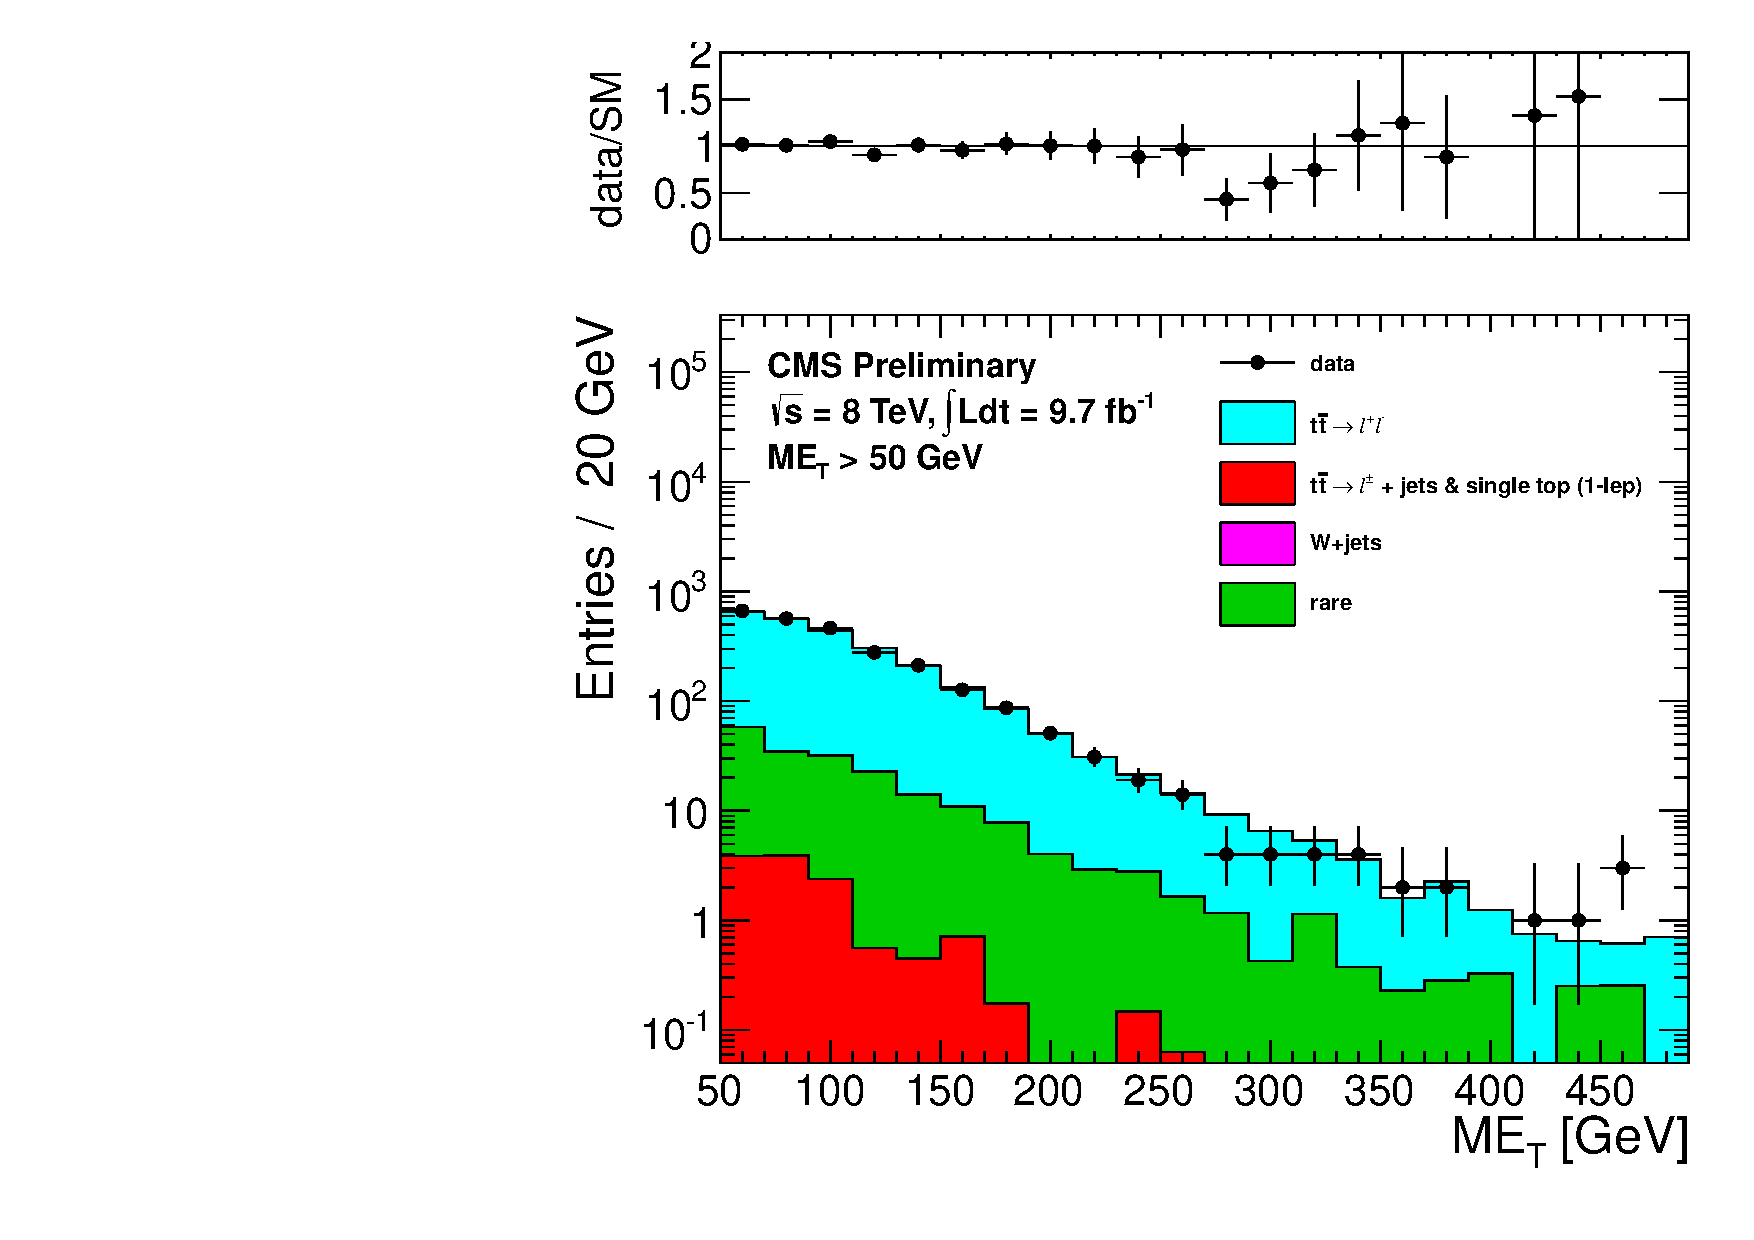
\includegraphics[width=0.5\linewidth]{plots/pas_log/met_met50_nj4_emucomb_CR4.pdf}%        
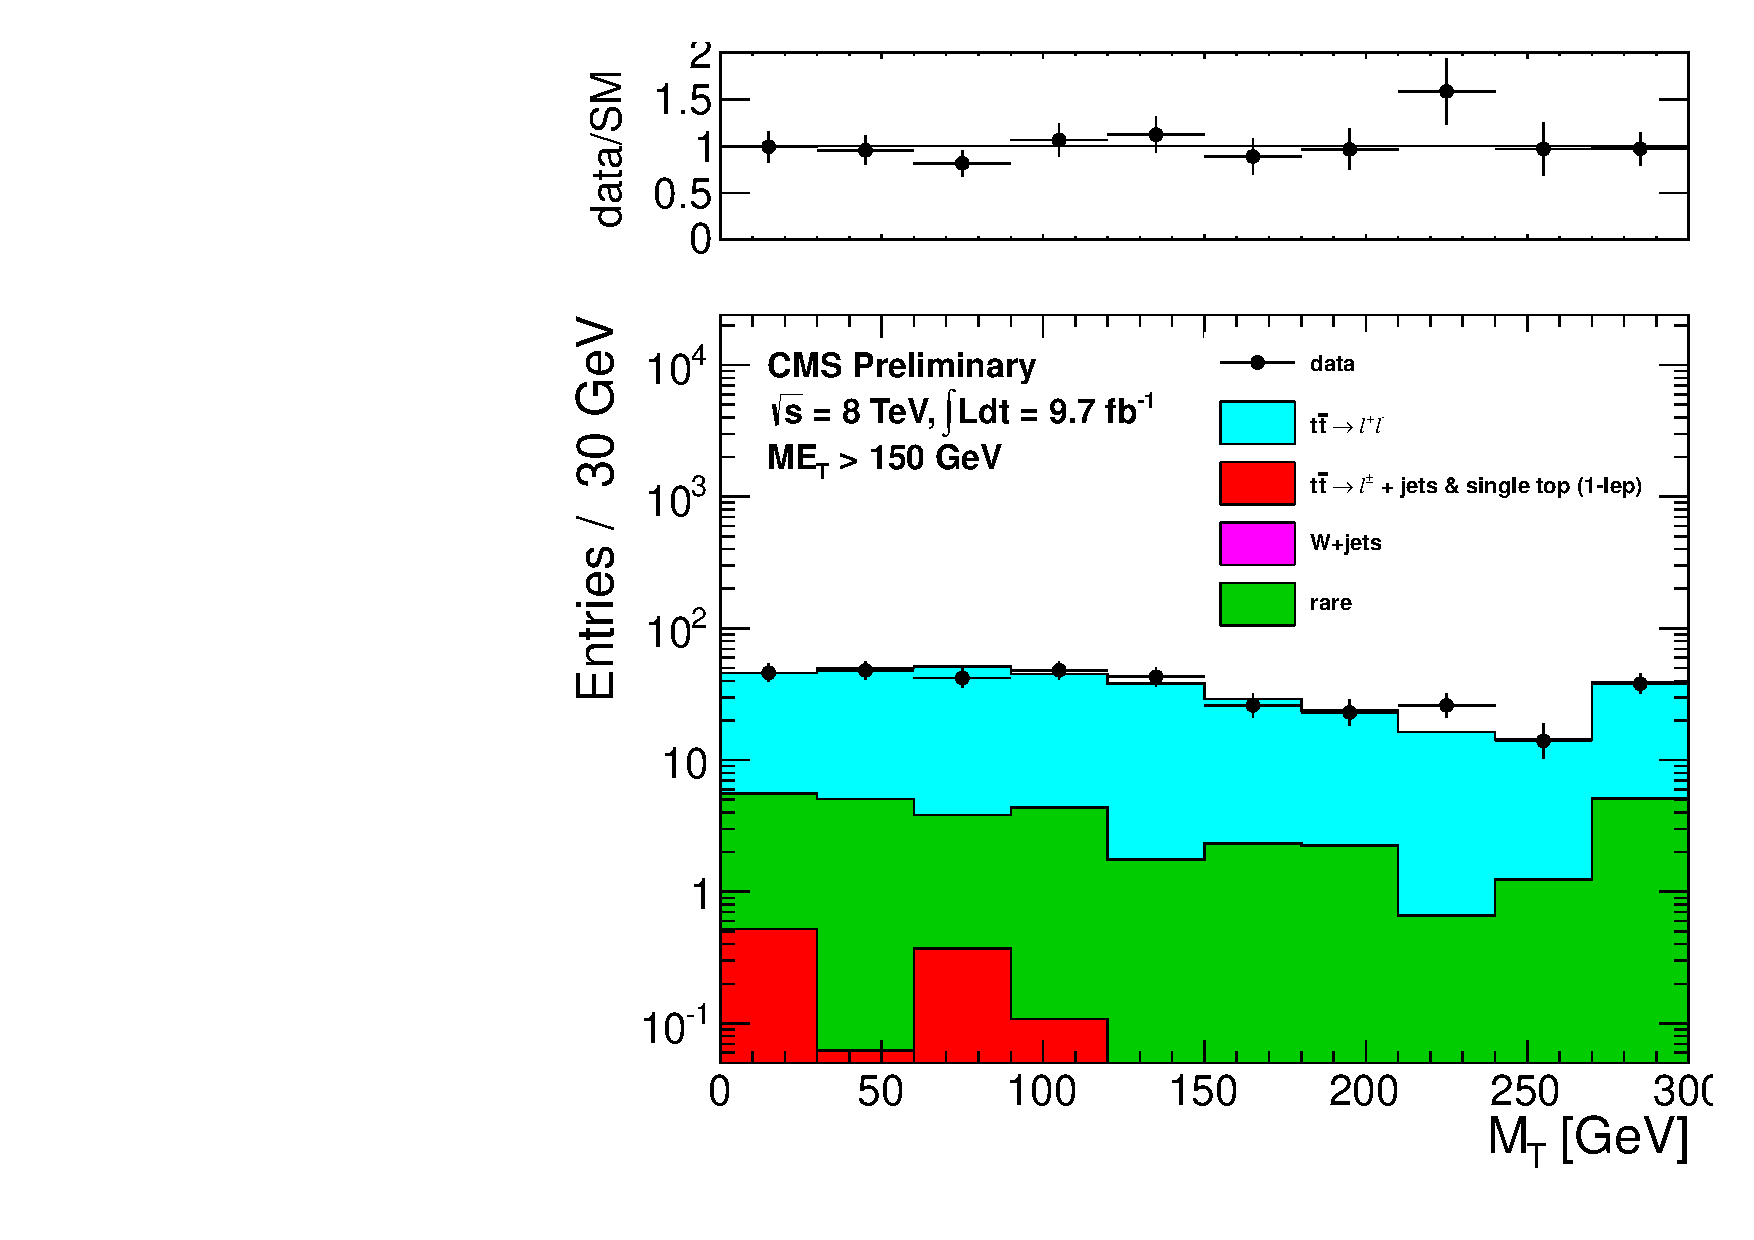
\includegraphics[width=0.5\linewidth]{plots/pas_log/mt_met150_nj4_emucomb_CR4.pdf}    
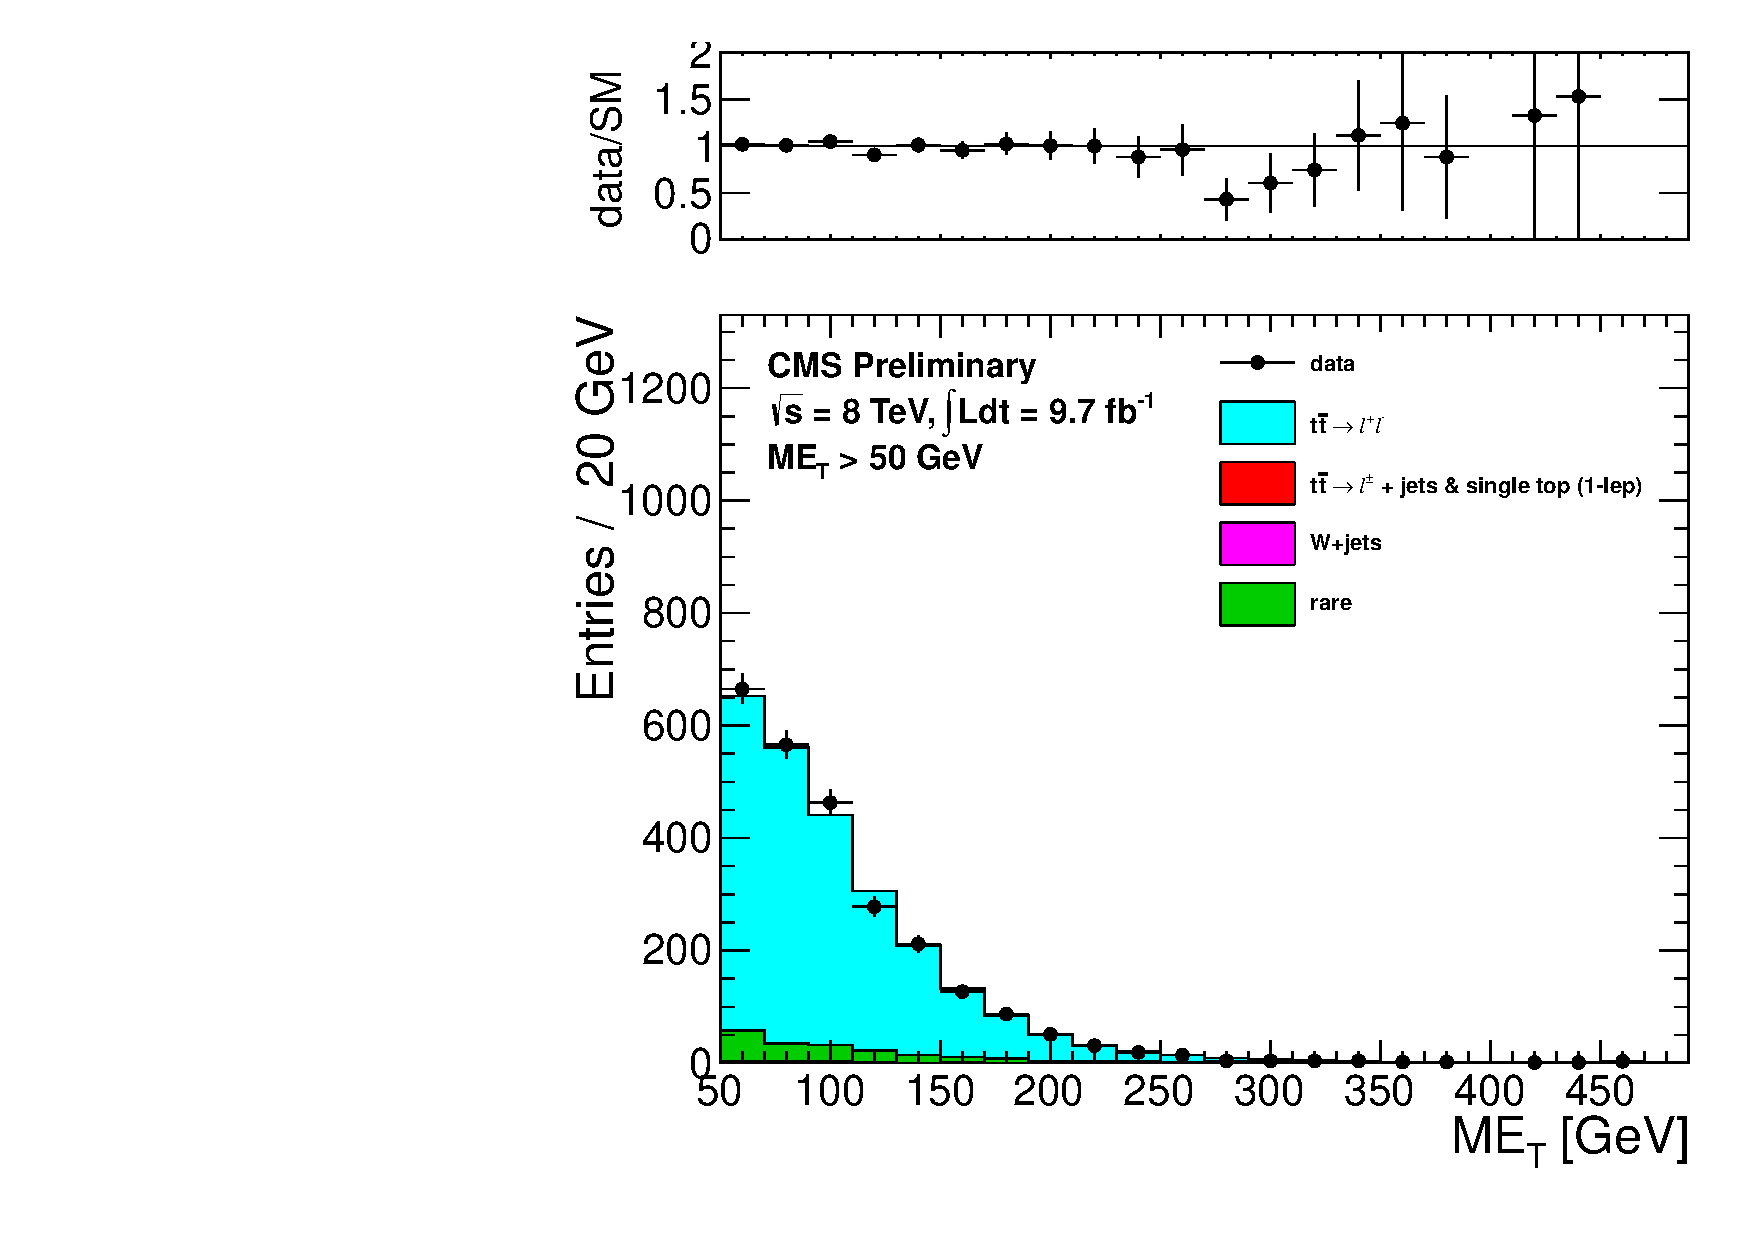
\includegraphics[width=0.5\linewidth]{plots/pas_lin/met_met50_nj4_emucomb_CR4.pdf}%        
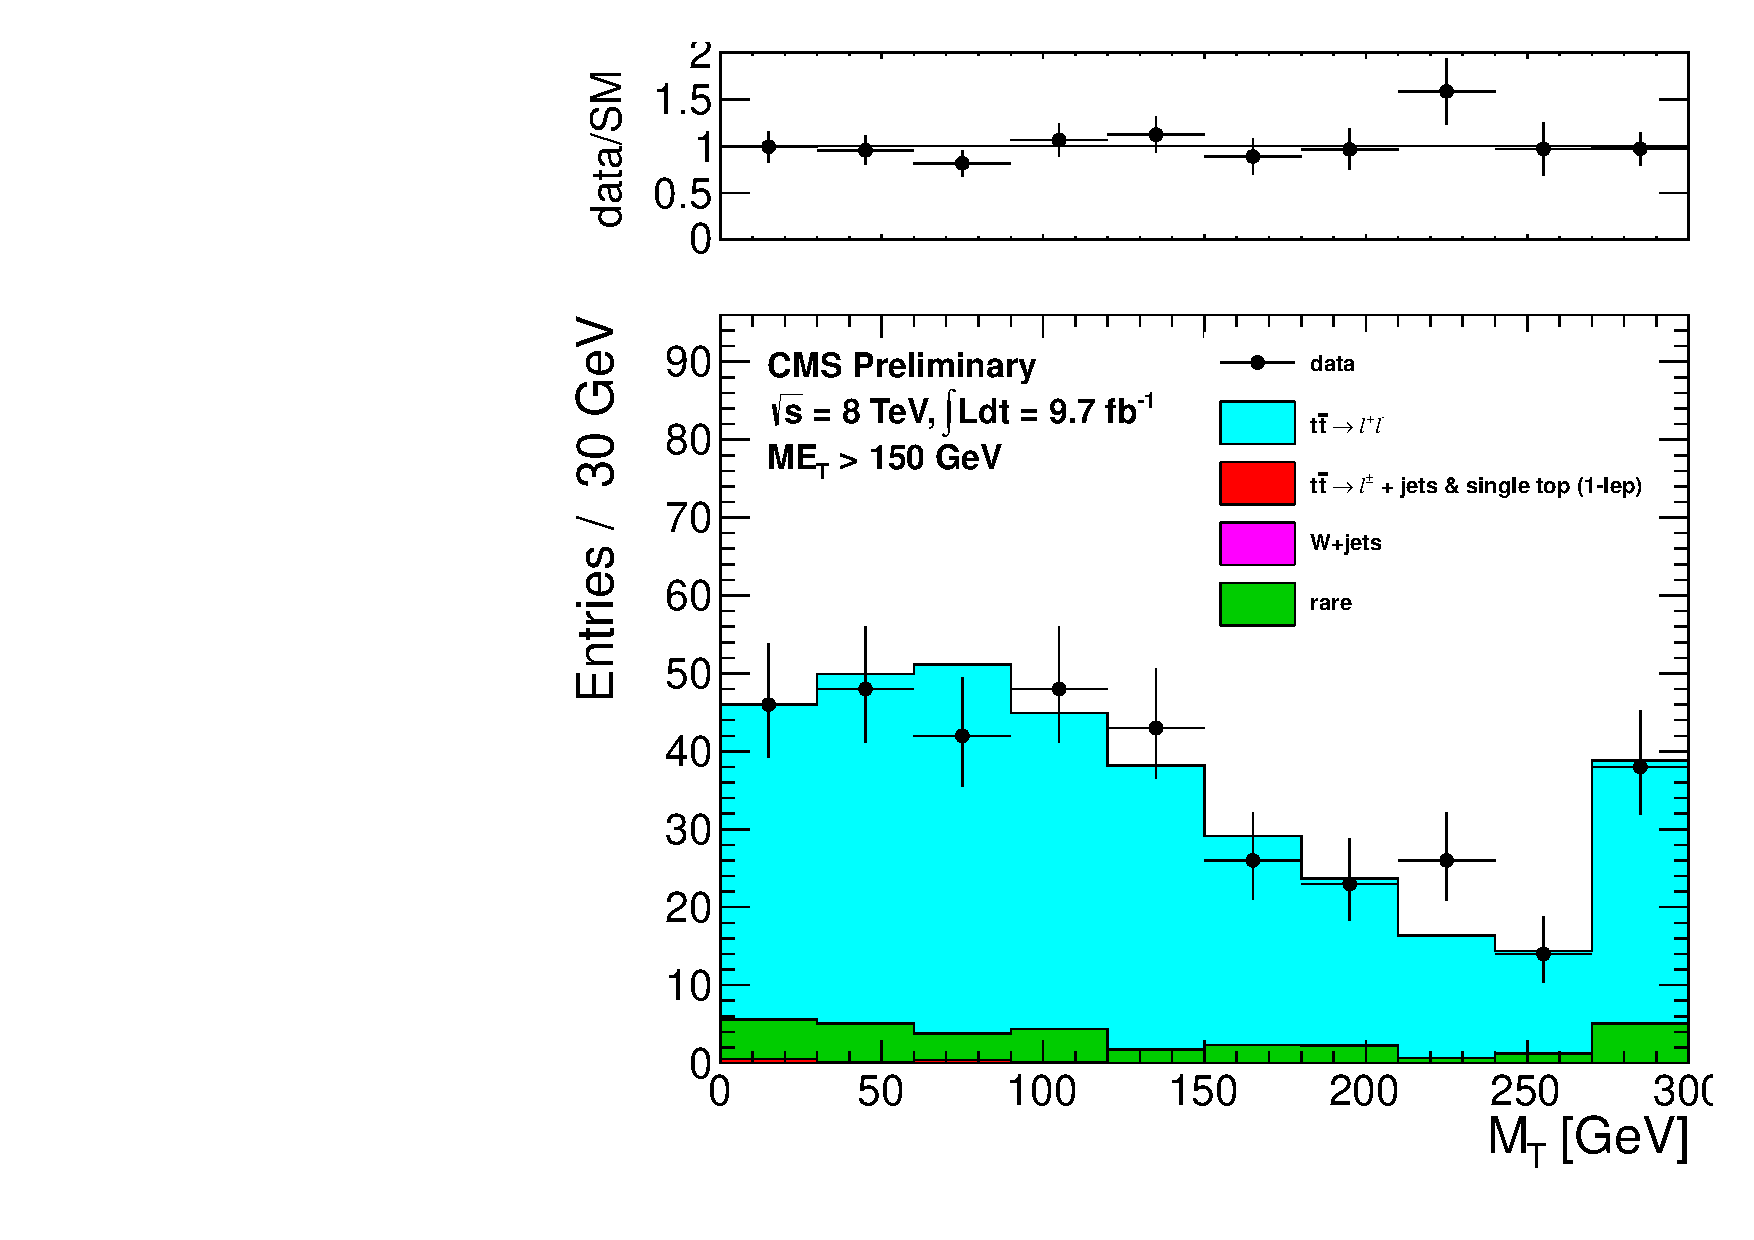
\includegraphics[width=0.5\linewidth]{plots/pas_lin/mt_met150_nj4_emucomb_CR4.pdf}    
\caption{
Comparison of the \met\ distribution (left) and \mt\ distribution for events satisfying \met\ $>$ 150 GeV (right)
in data vs. MC for CR4. 
\label{fig:cr4met}} 
\end{center}
\end{figure} 
  
\clearpage

\subsection {CR5: $\ge$ 1 b-tag, 1 lepton + 1 isolated track}
\label{sec:CR5}

\begin{figure}[hbt]
  \begin{center}
        %\includegraphics[width=0.5\linewidth]{plots/CR5_met_met50_leadmuo_nj4.pdf}%
        %\includegraphics[width=0.5\linewidth]{plots/CR5_met_met50_leadele_nj4.pdf}
        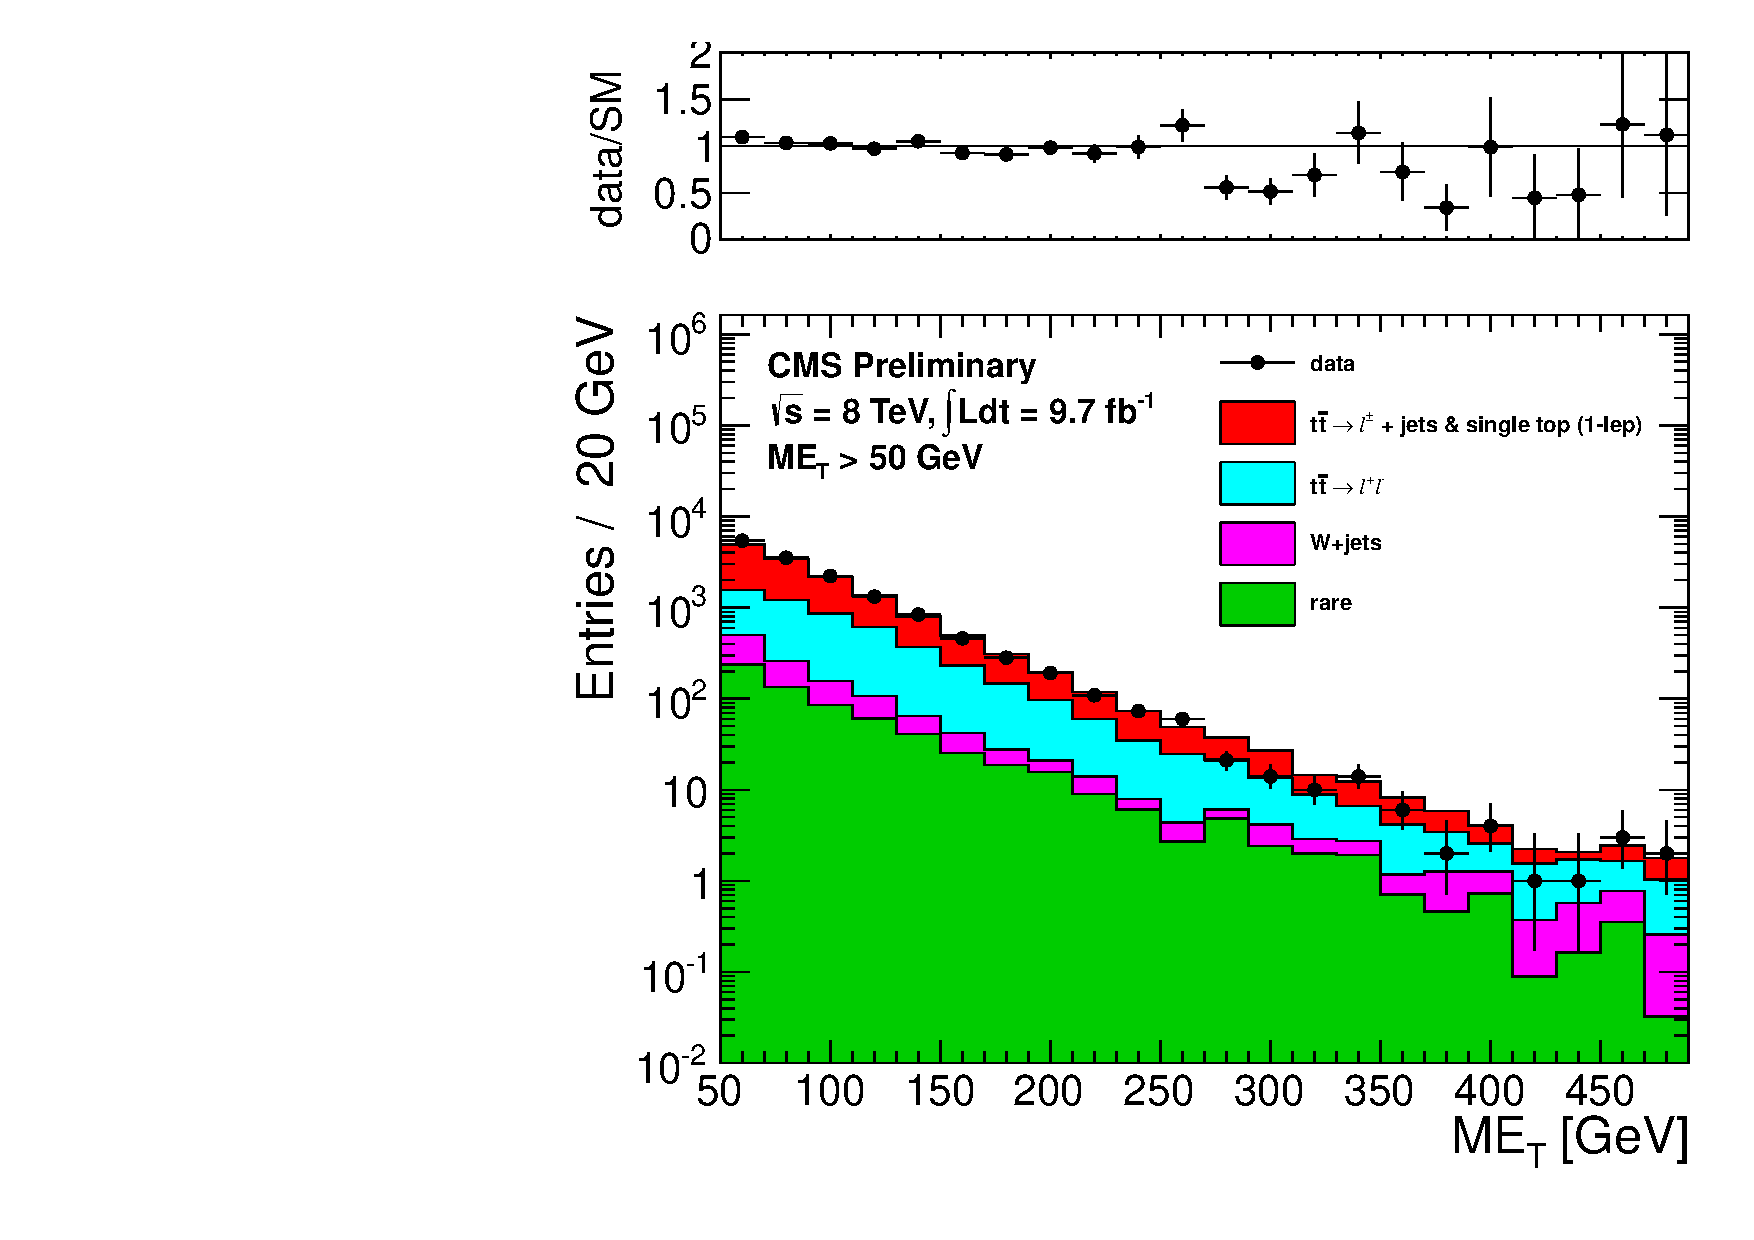
\includegraphics[width=0.5\linewidth]{plots/pas_log/met_met50_nj4_emucomb_CR5.pdf}%
        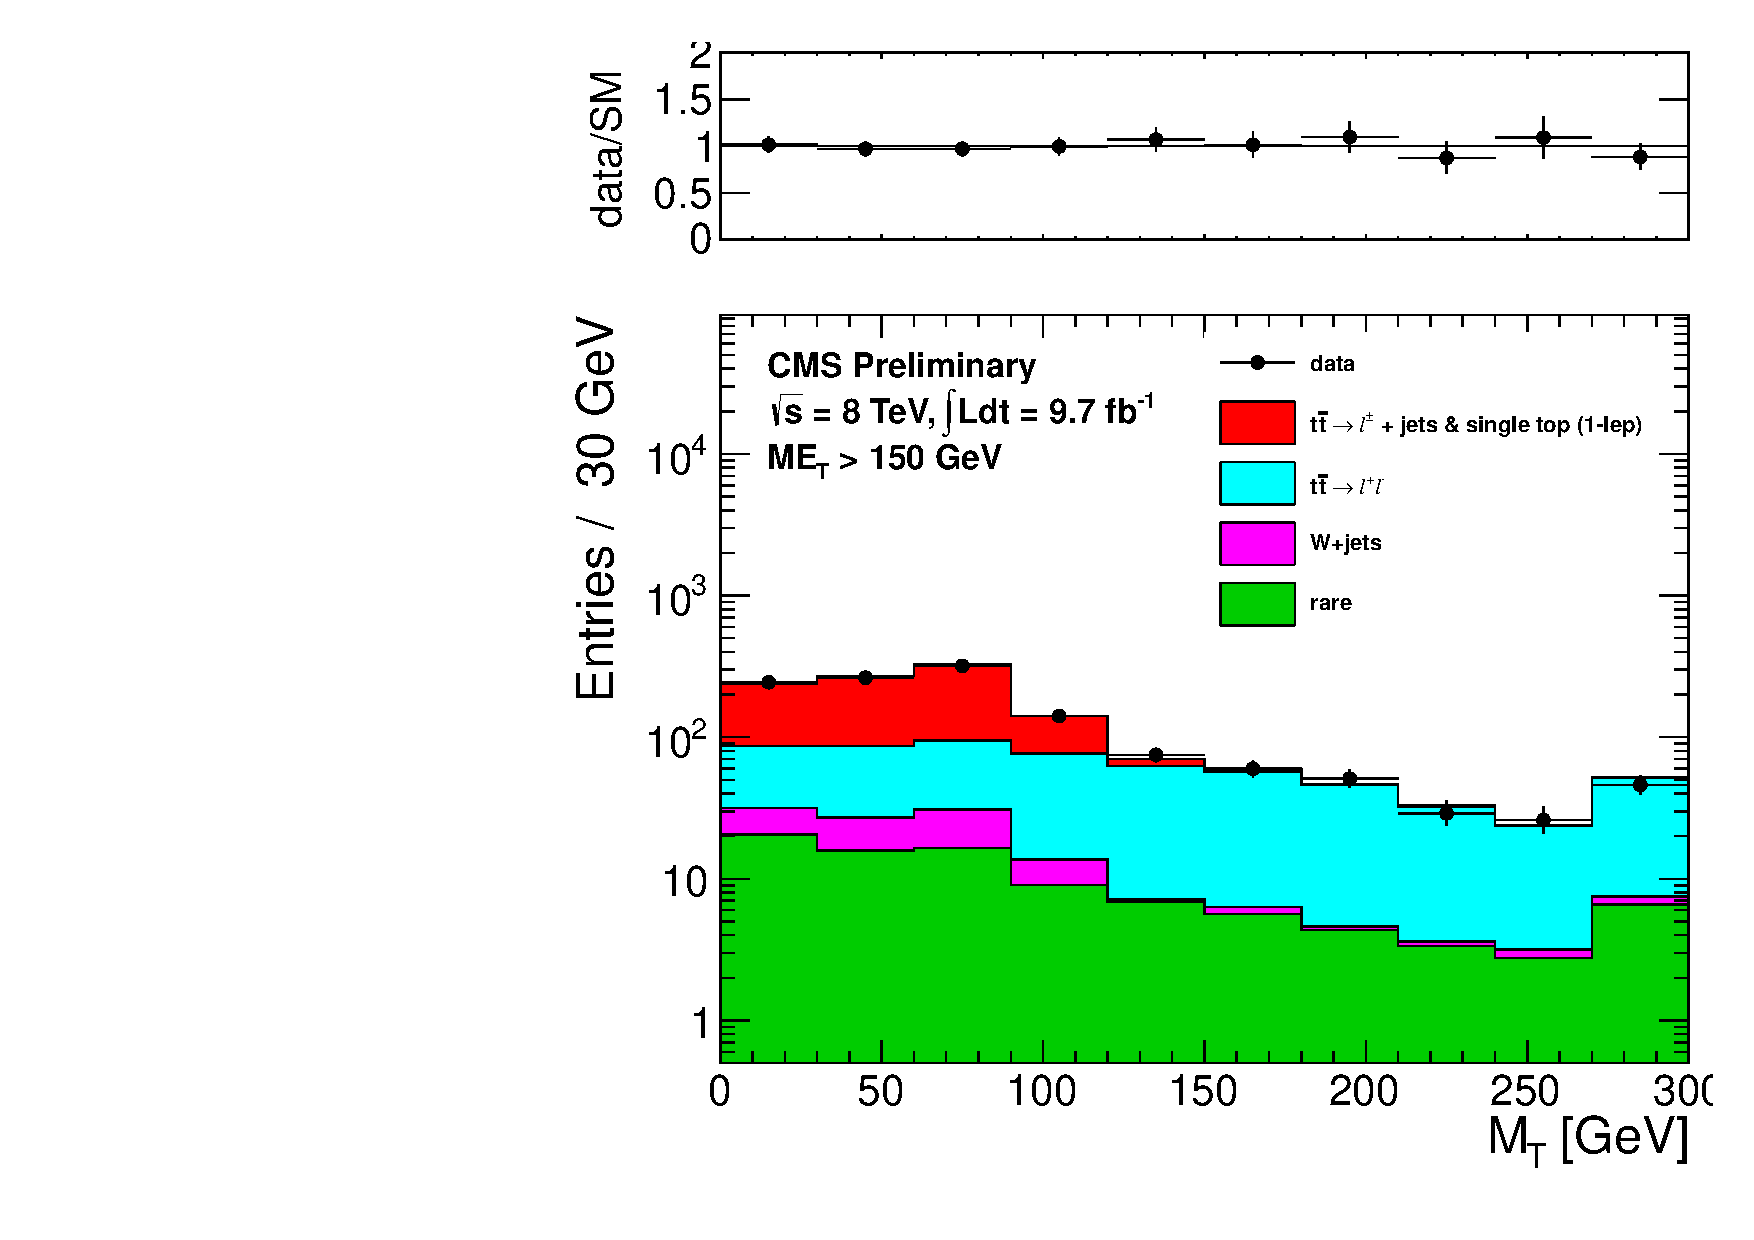
\includegraphics[width=0.5\linewidth]{plots/pas_log/mt_met150_nj4_emucomb_CR5.pdf}
        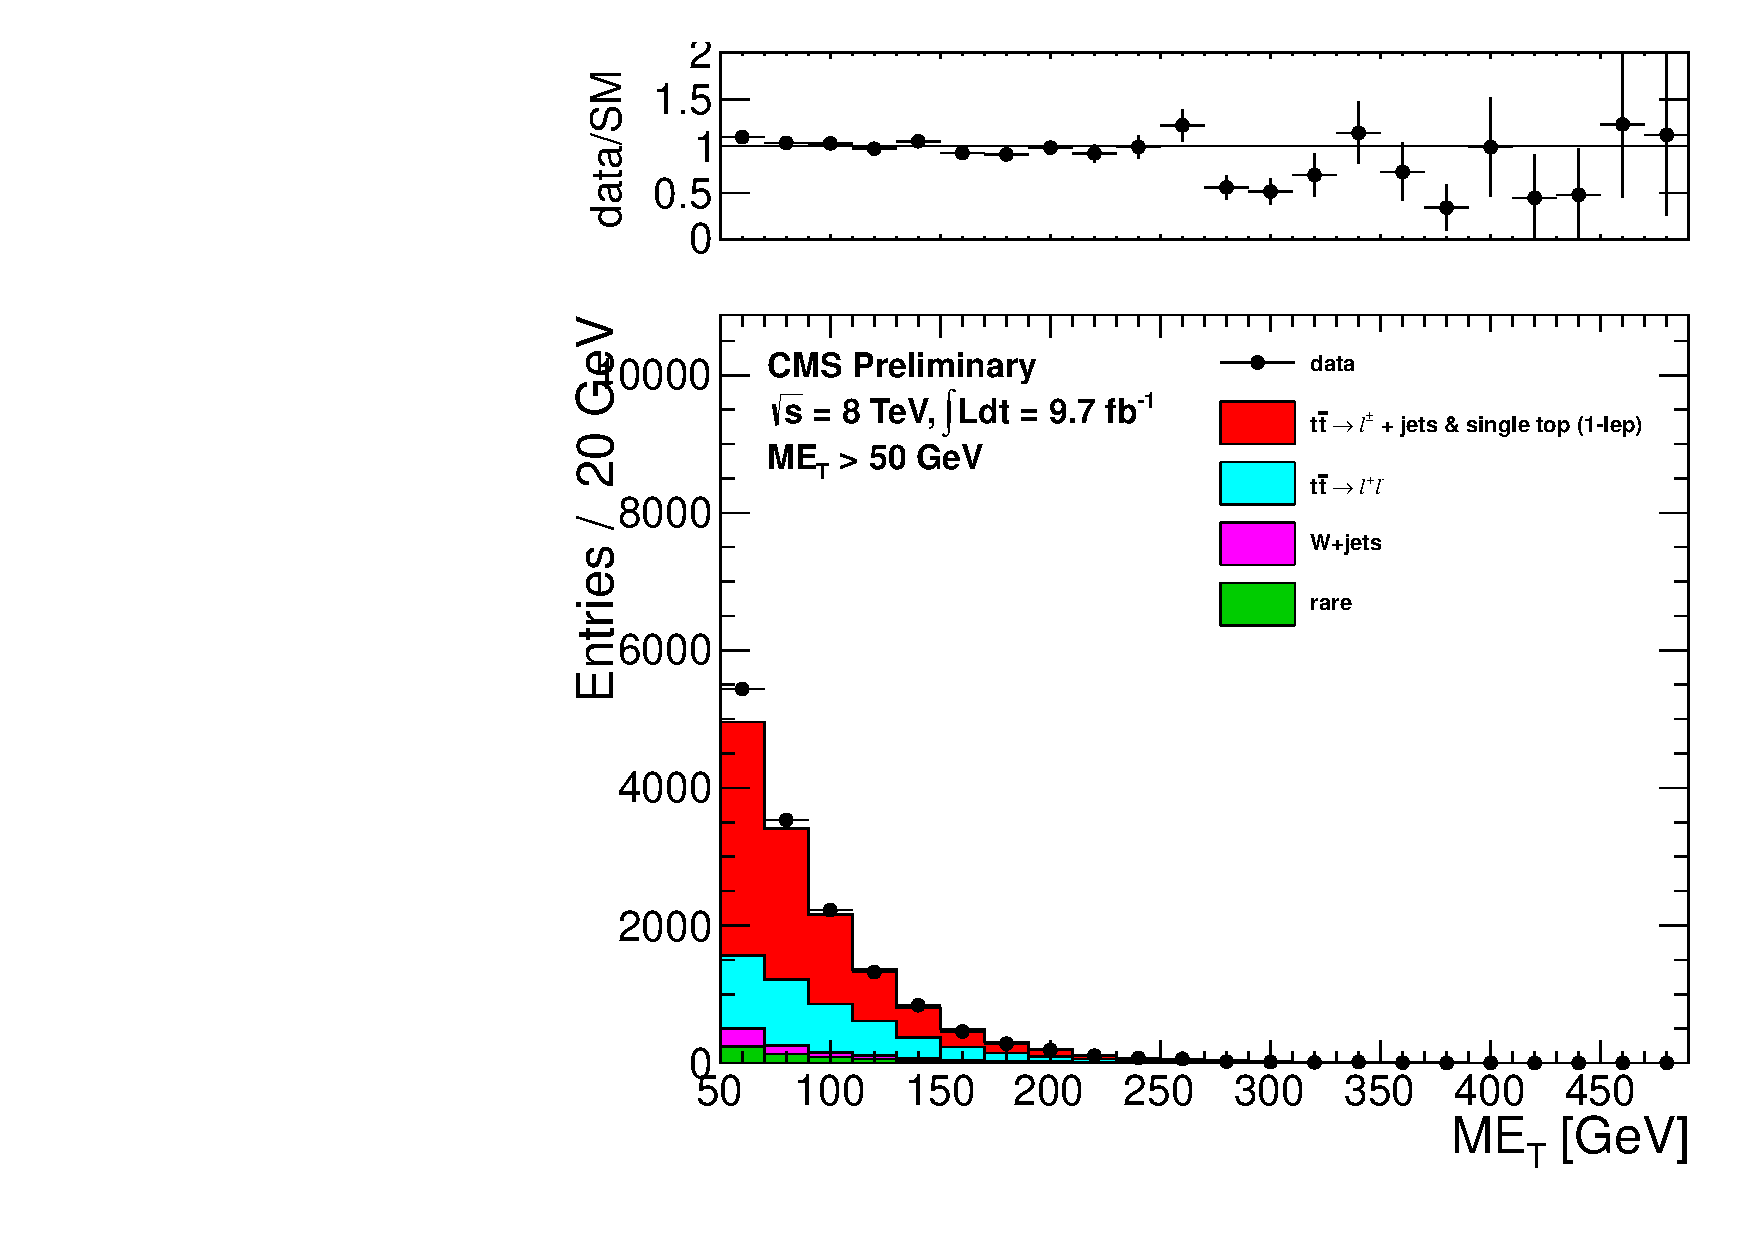
\includegraphics[width=0.5\linewidth]{plots/pas_lin/met_met50_nj4_emucomb_CR5.pdf}%
        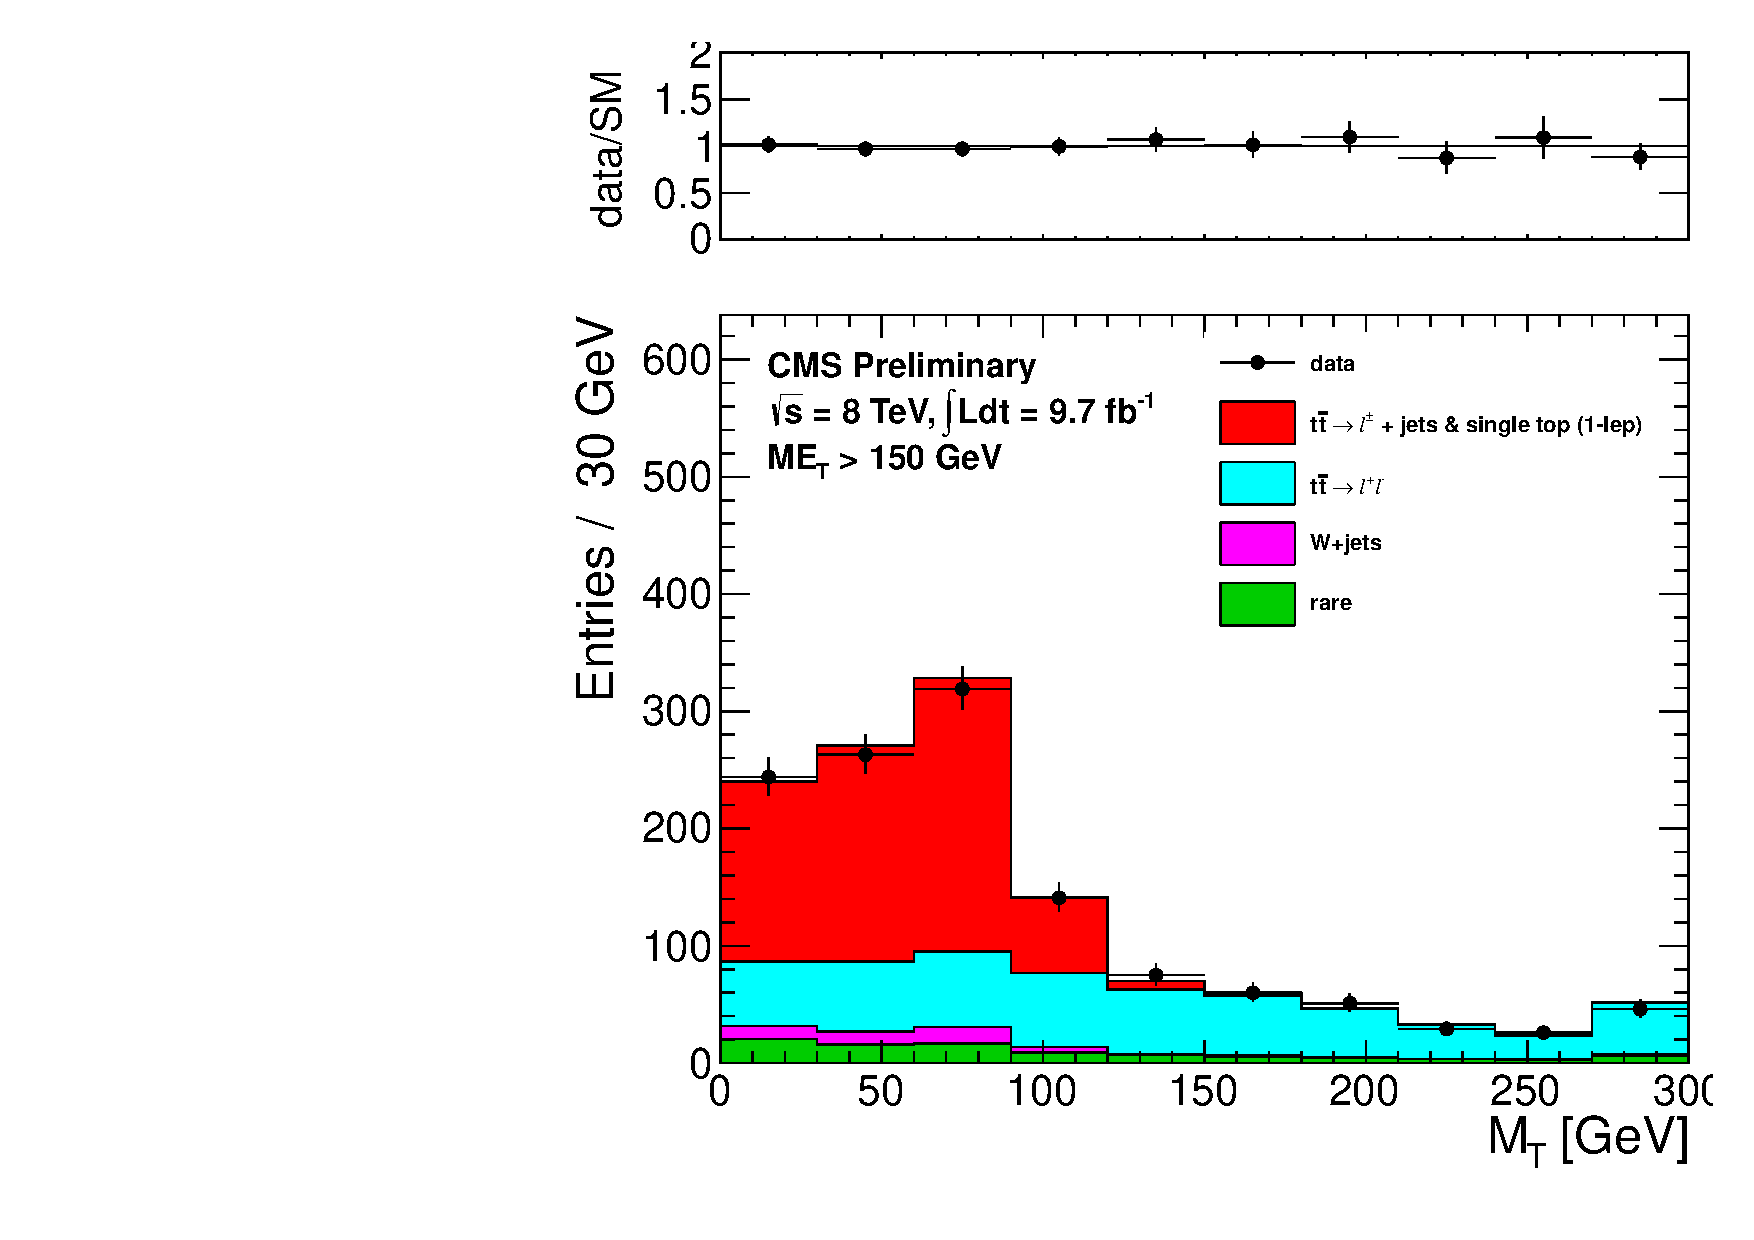
\includegraphics[width=0.5\linewidth]{plots/pas_lin/mt_met150_nj4_emucomb_CR5.pdf}
    \caption{
Comparison of the \met\ distribution (left) and \mt\ distribution for events satisfying \met\ $>$ 150 GeV (right)
in data vs. MC for CR5. 
\label{fig:cr5met} 
}  
      \end{center}
\end{figure}

\clearpage

 \subsection {CR1: 0 b-tags, exactly 1 lepton}
 \label{sec:cr1}

 \begin{figure}[hbt]
  \begin{center}
        %\includegraphics[width=0.5\linewidth]{plots/CR1_met_met50_leadmuo_nj4.pdf}%
        %\includegraphics[width=0.5\linewidth]{plots/CR1_met_met50_leadele_nj4.pdf}
        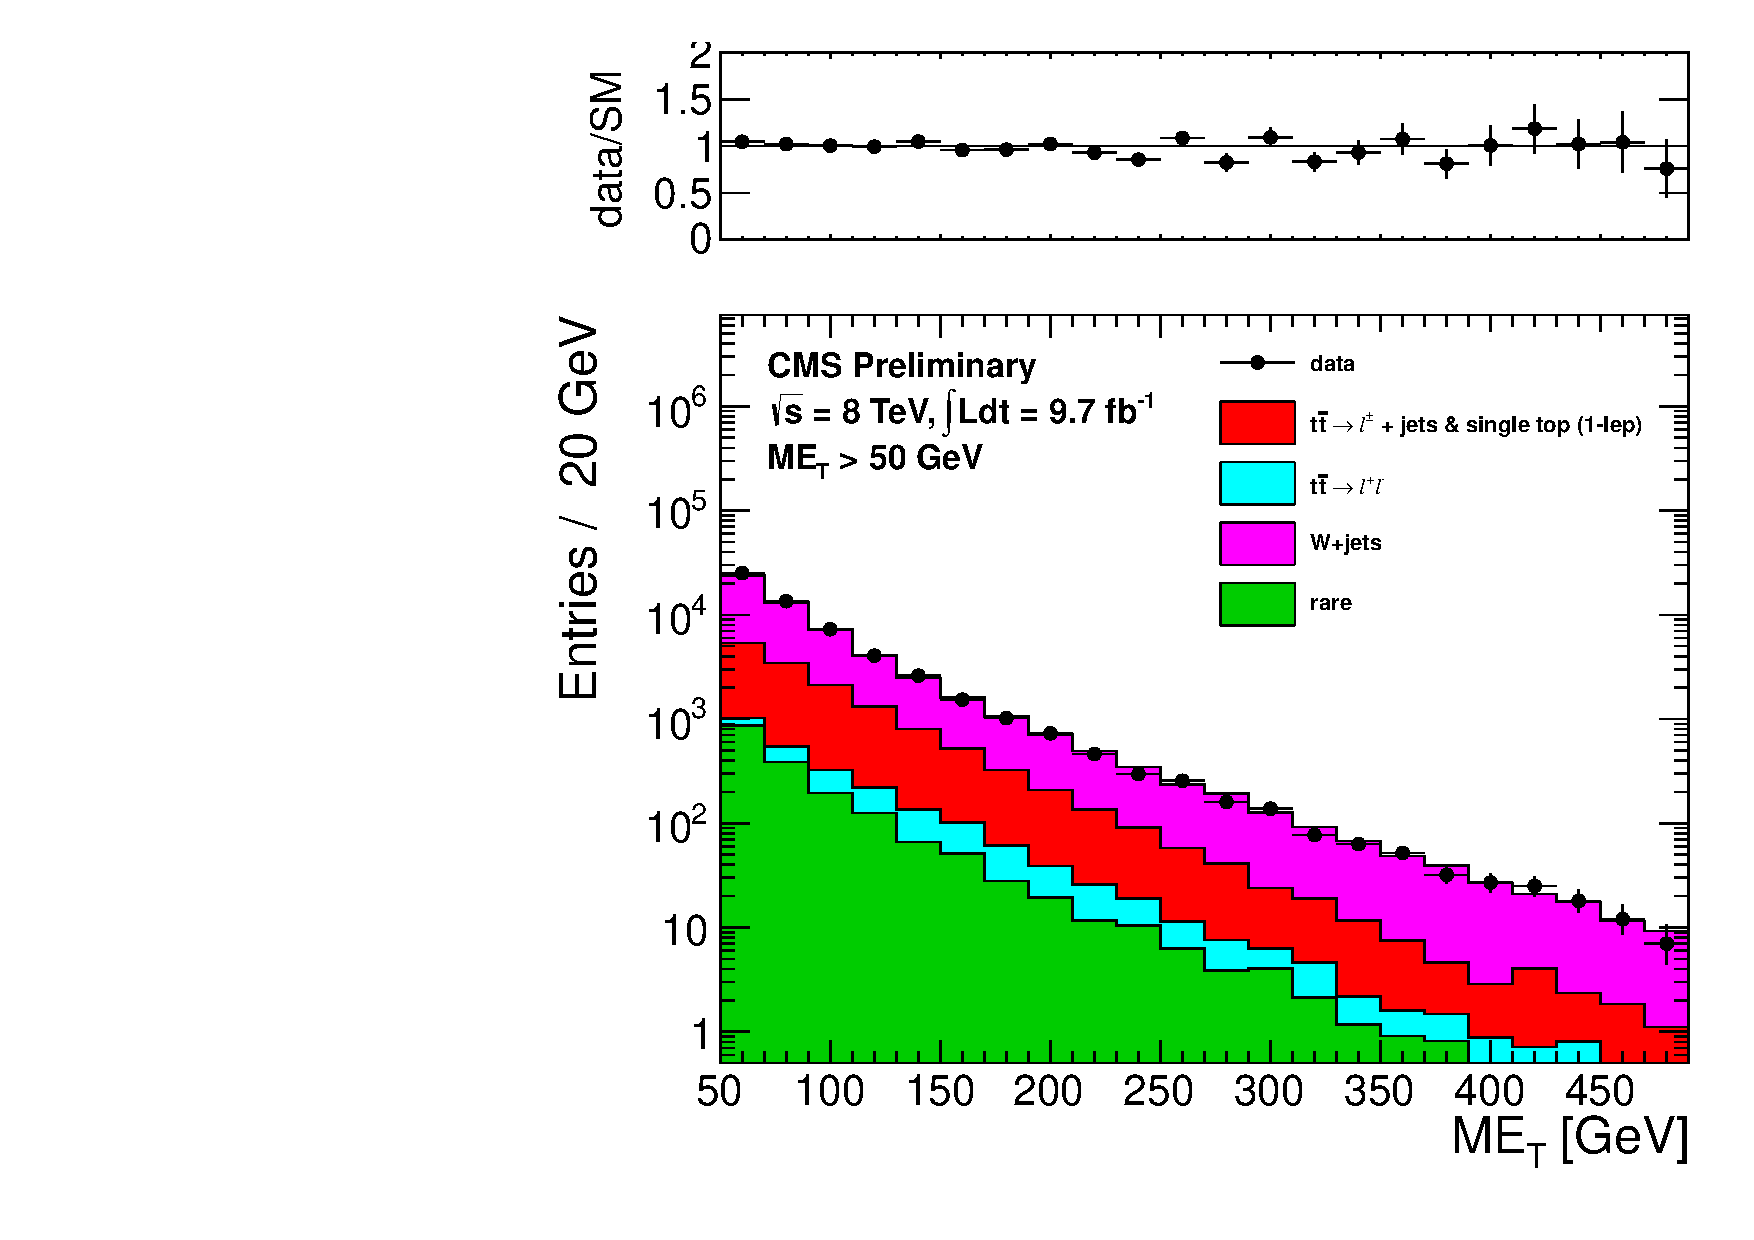
\includegraphics[width=0.5\linewidth]{plots/pas_log/met_met50_nj4_emucomb_CR1.pdf}%
        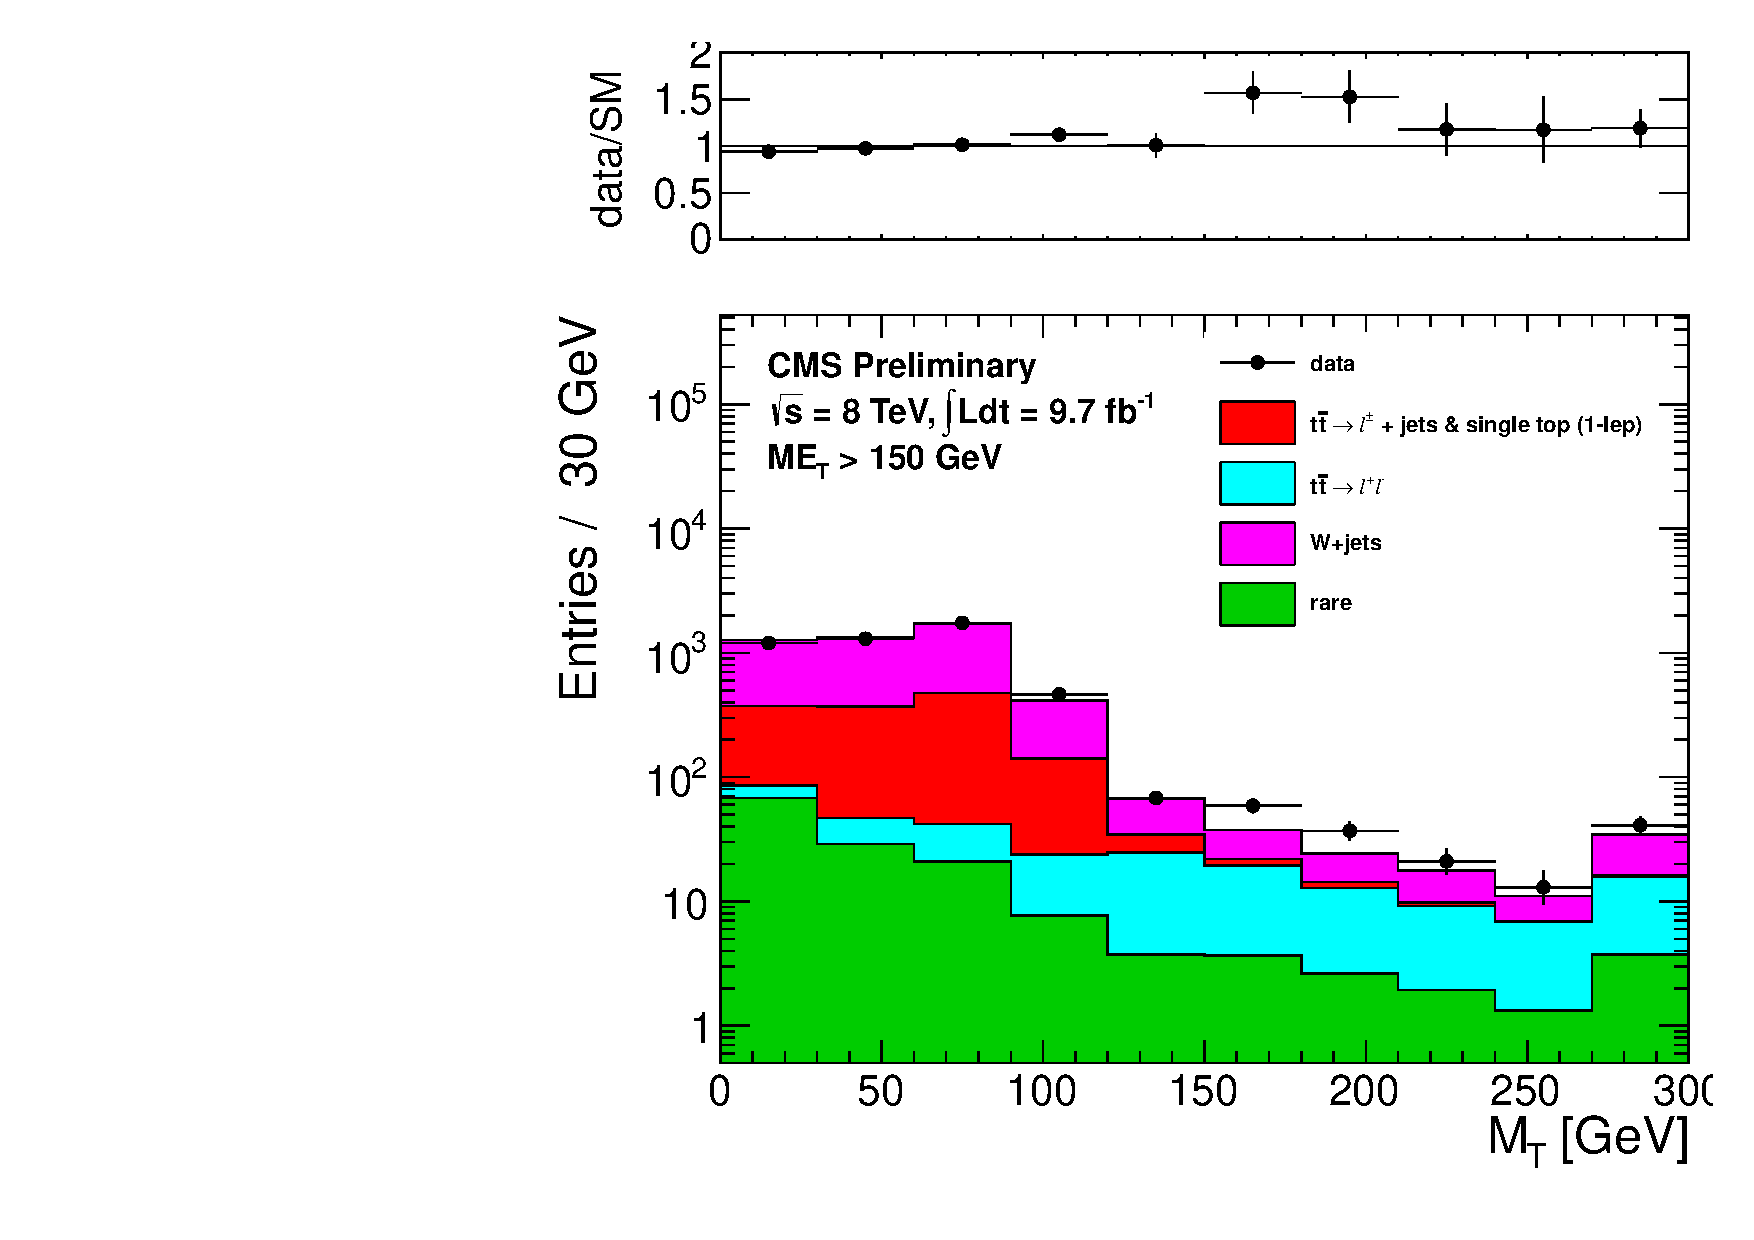
\includegraphics[width=0.5\linewidth]{plots/pas_log/mt_met150_nj4_emucomb_CR1.pdf}
        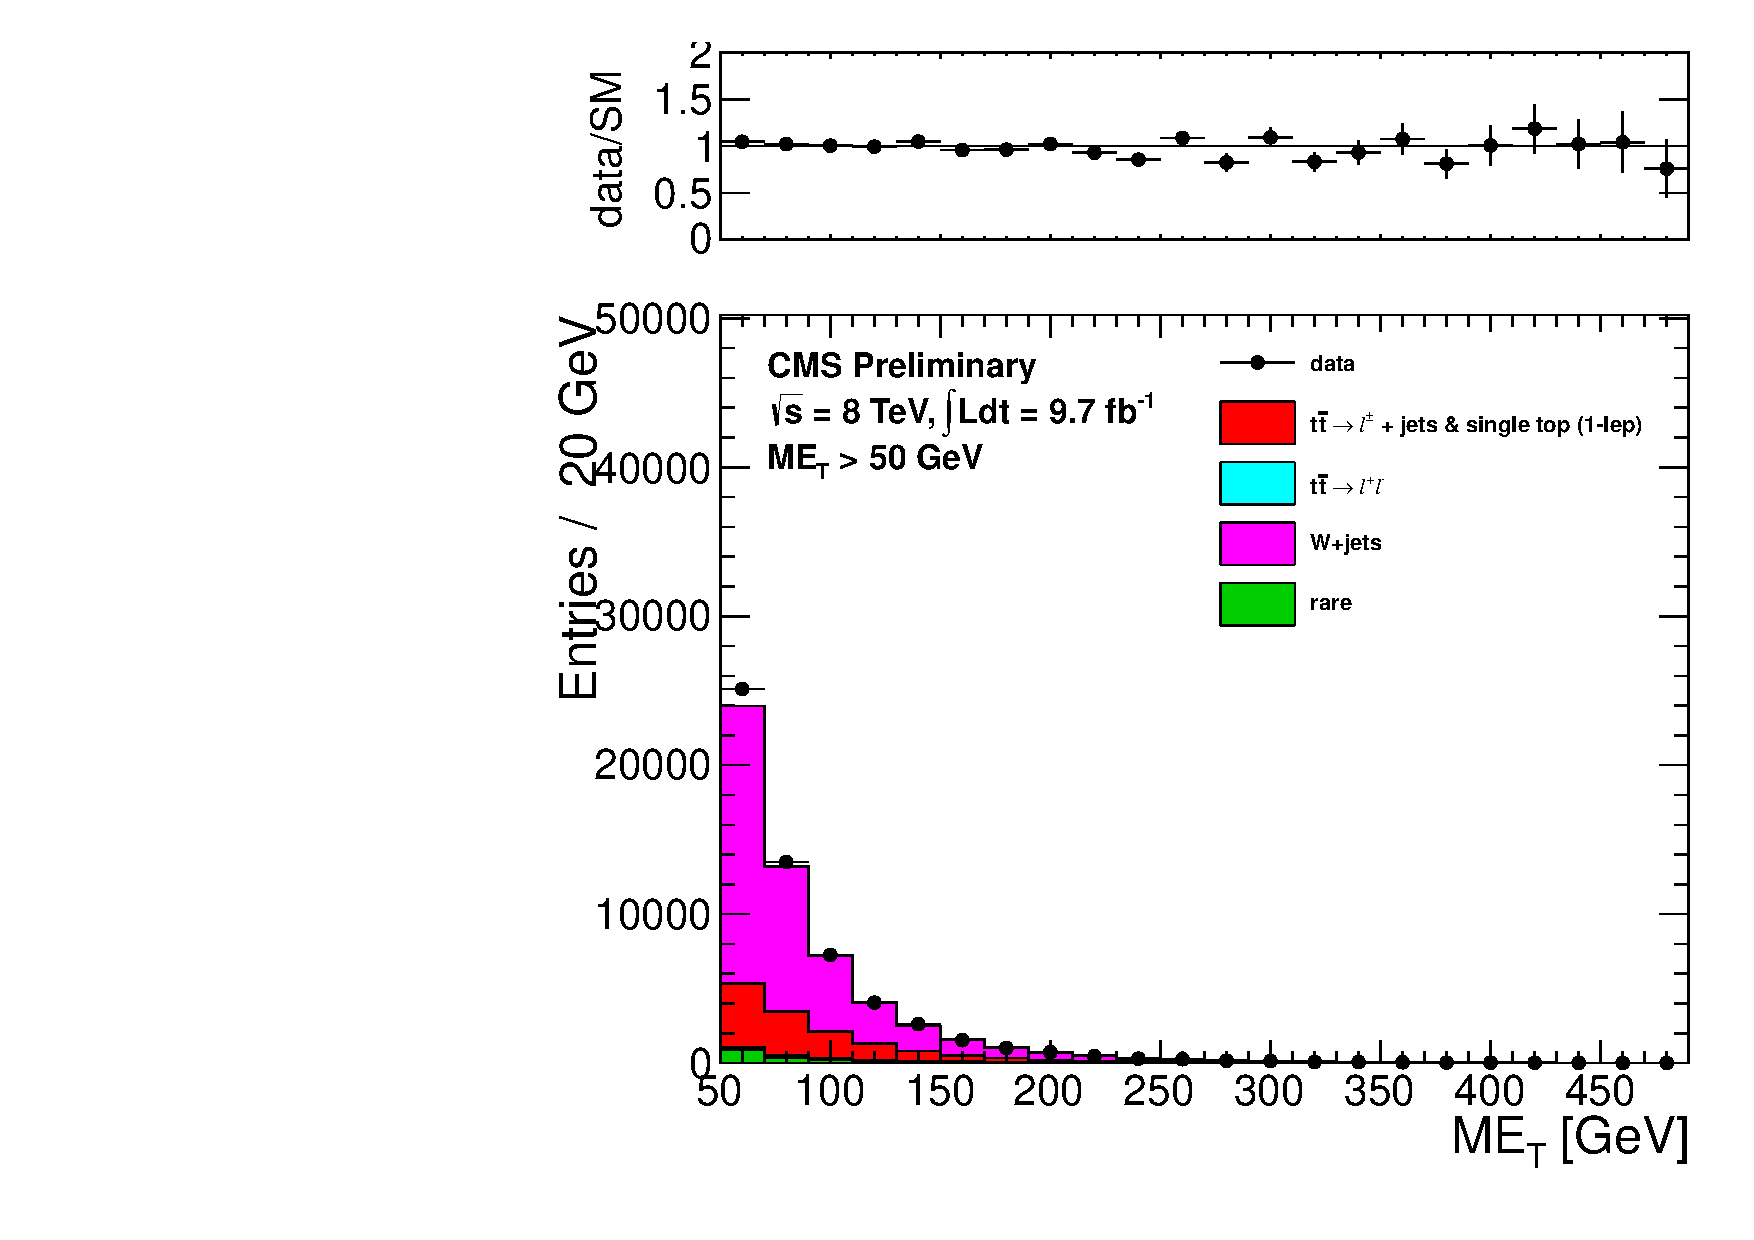
\includegraphics[width=0.5\linewidth]{plots/pas_lin/met_met50_nj4_emucomb_CR1.pdf}%
        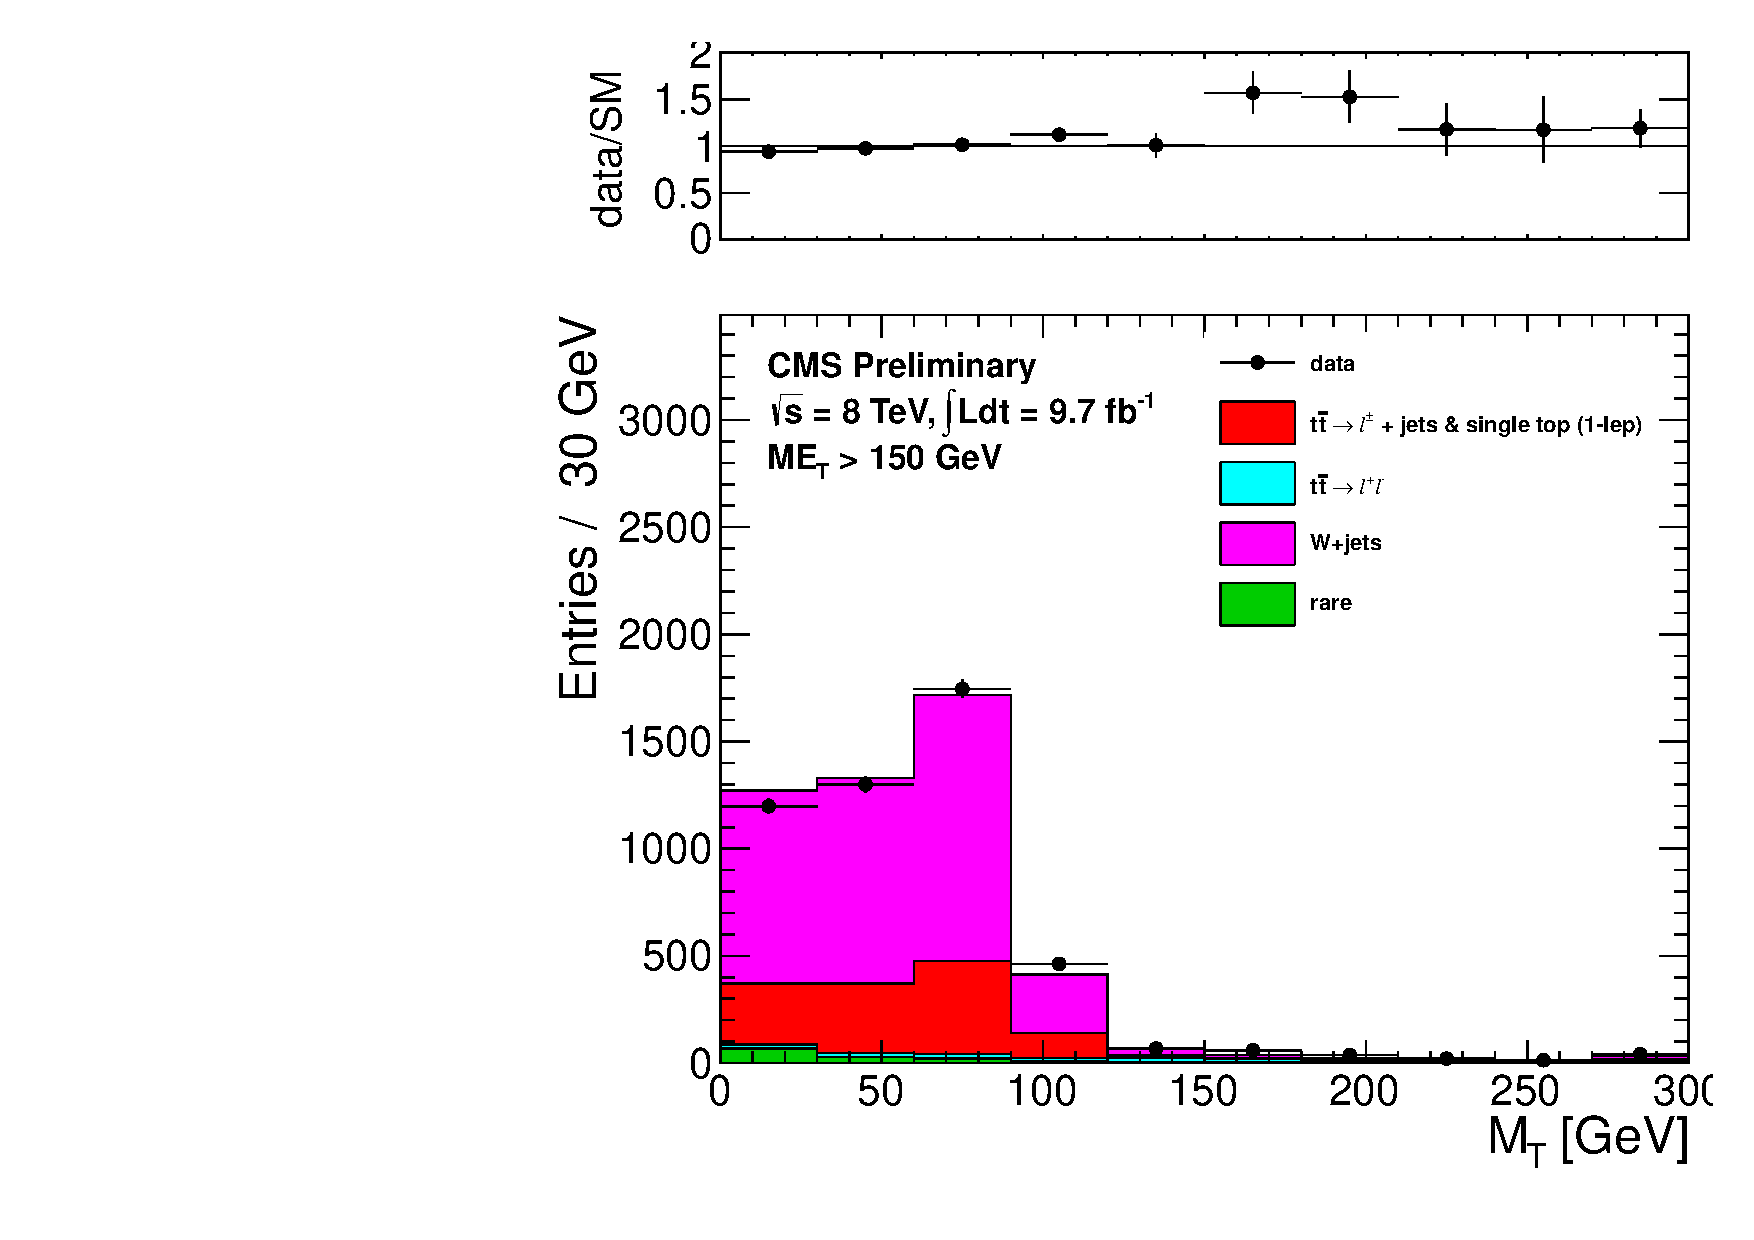
\includegraphics[width=0.5\linewidth]{plots/pas_lin/mt_met150_nj4_emucomb_CR1.pdf}
    \caption{
      Comparison of the \met\ distribution (left) and the \mt\ distribution after a \met\ $>$ 150 GeV requirement (right)
      in data vs. MC for events satisfying the requirements of CR1.
\label{fig:cr1met} 
}  
 \end{center}
\end{figure}

\clearpage

 \subsection {CR2: 0 b-tags, exactly 2 leptons}

 \begin{figure}[hbt]
   \begin{center}
     %\includegraphics[width=0.5\linewidth]{plots/CR2_met_lepcor_scaled_nj4_emucomb.pdf}%
     %\includegraphics[width=0.5\linewidth]{plots/CR2_mt_lepcor_scaled_nj4_emucomb.pdf}
     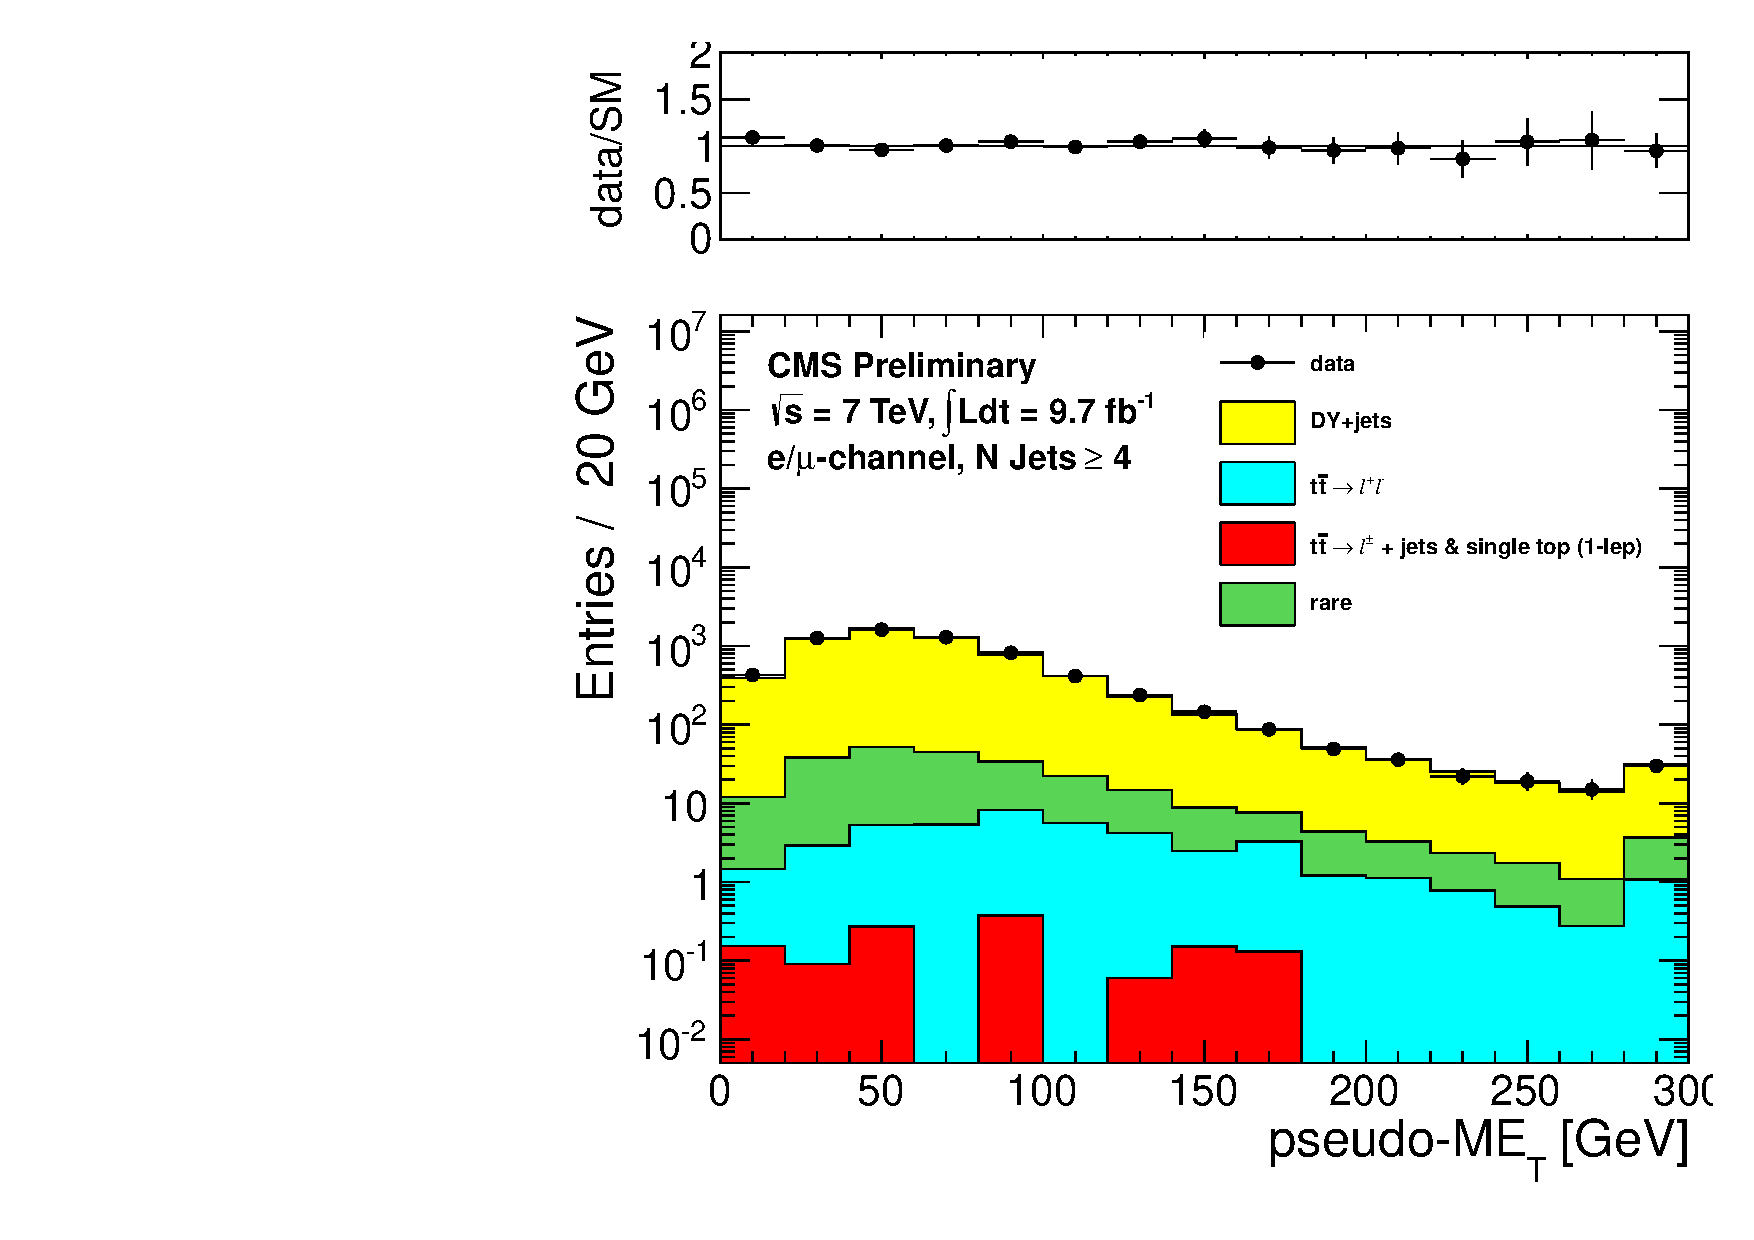
\includegraphics[width=0.5\linewidth]{plots/pas_log/met_lepcor_scaled_nj4_emucomb_CR2.pdf}%
     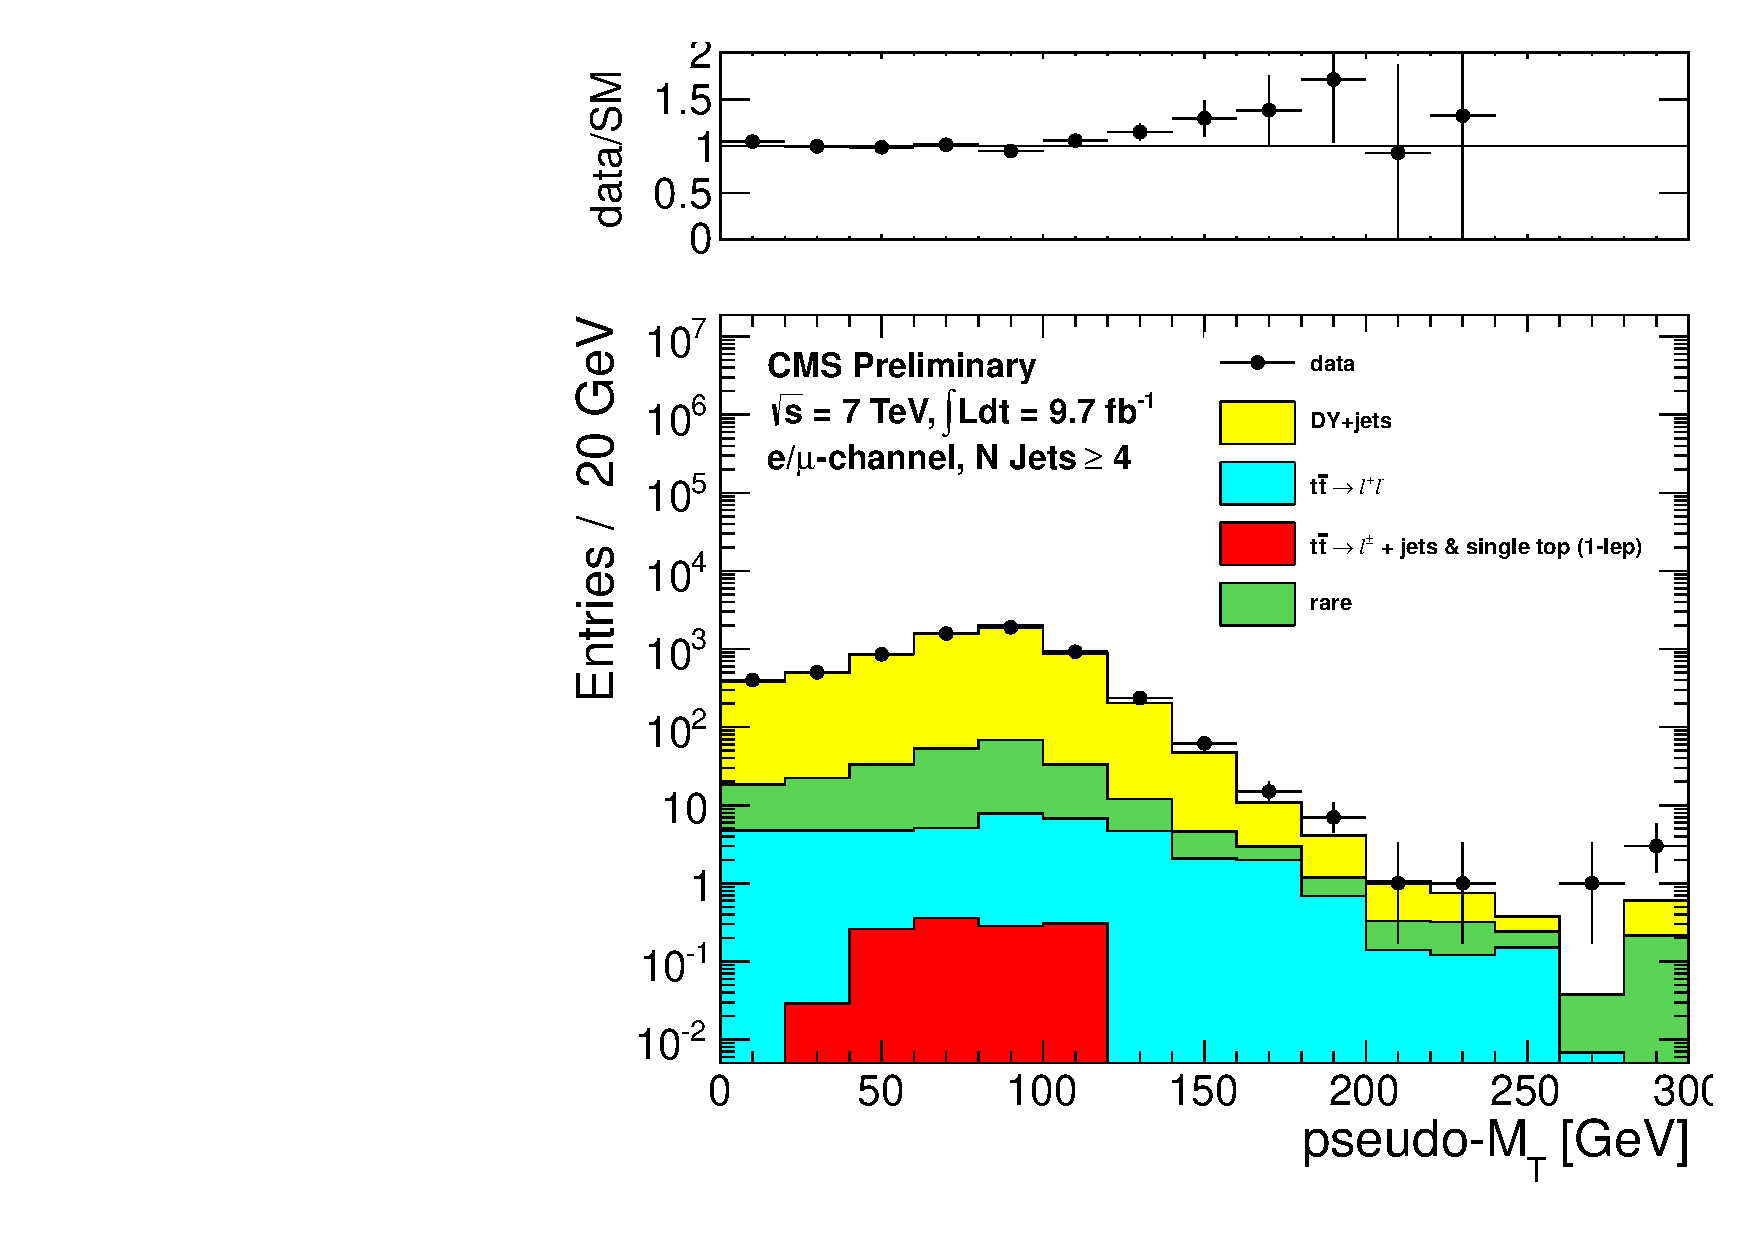
\includegraphics[width=0.5\linewidth]{plots/pas_log/mt_lepcor_scaled_nj4_emucomb_CR2.pdf}
     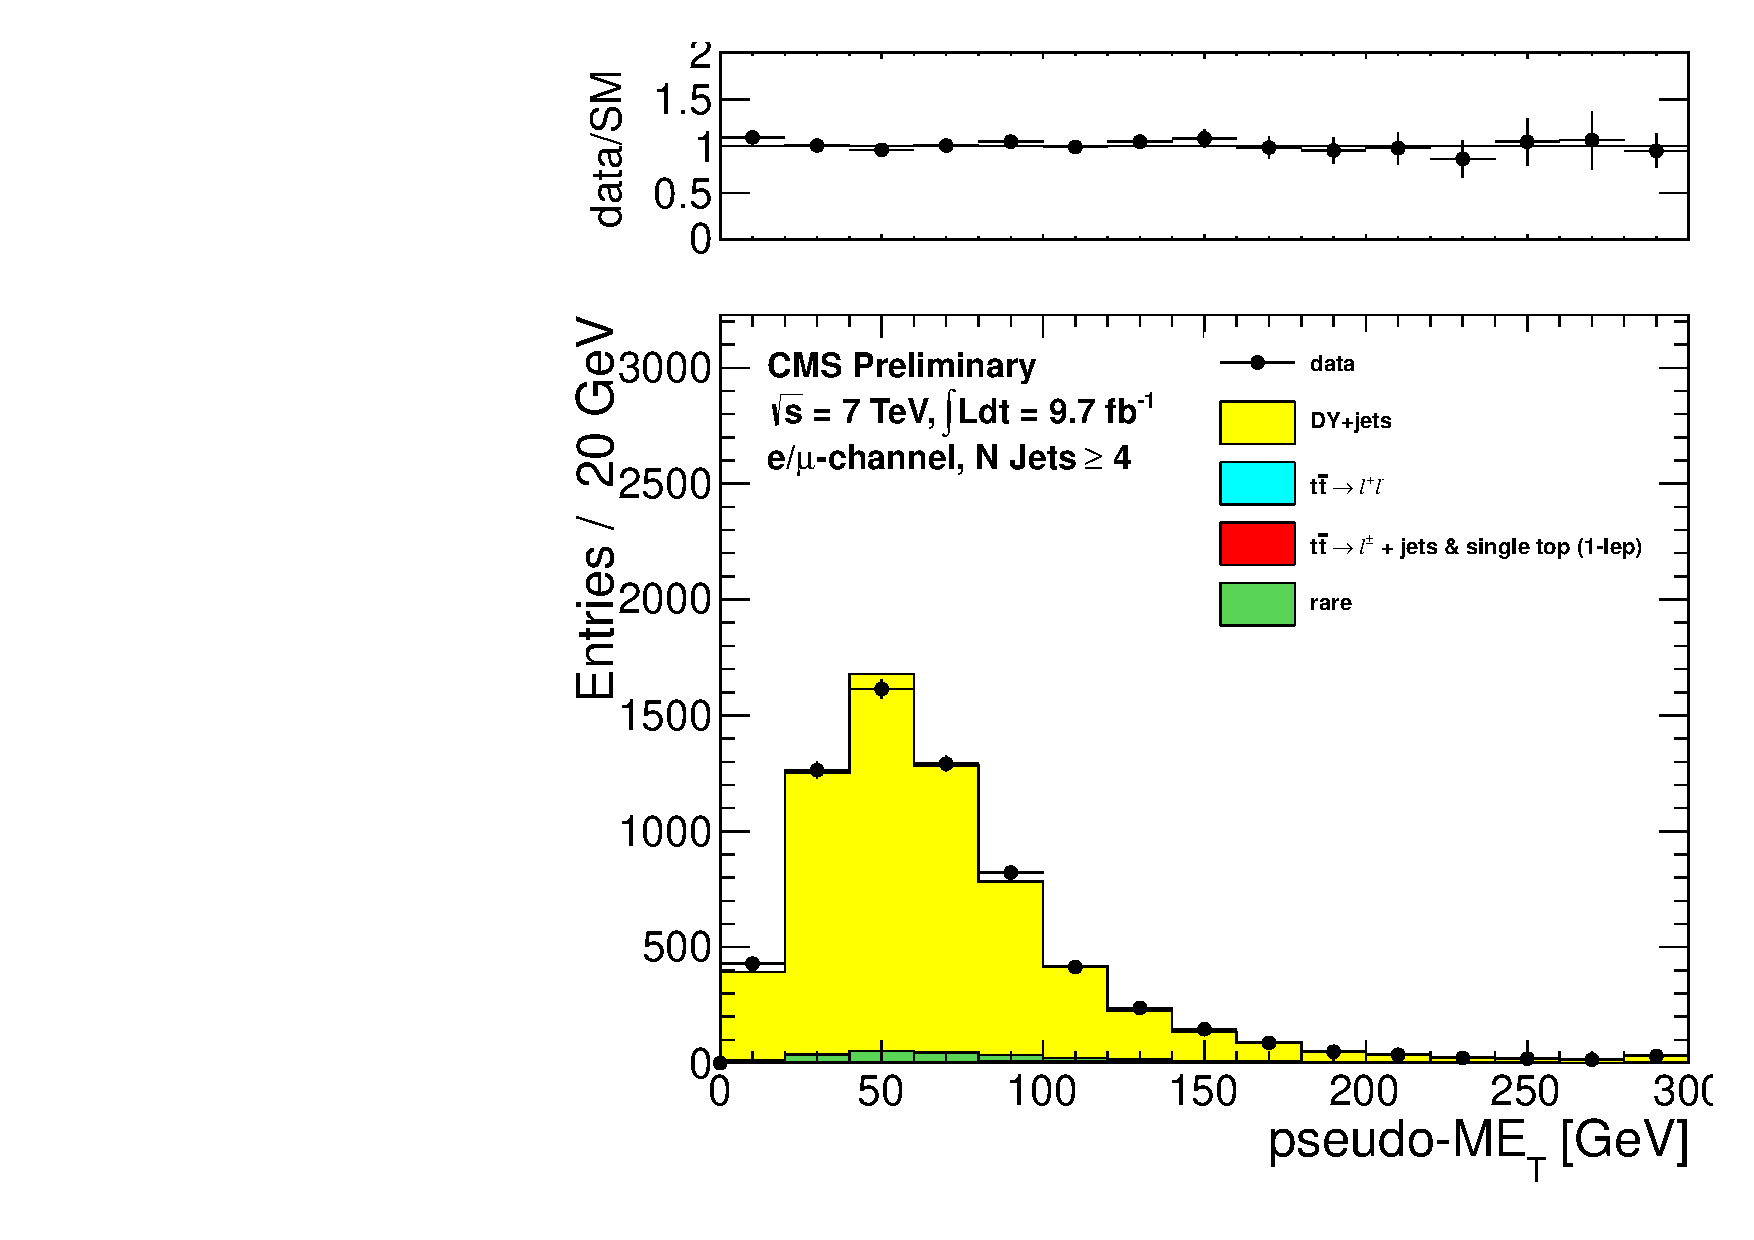
\includegraphics[width=0.5\linewidth]{plots/pas_lin/met_lepcor_scaled_nj4_emucomb_CR2.pdf}%
     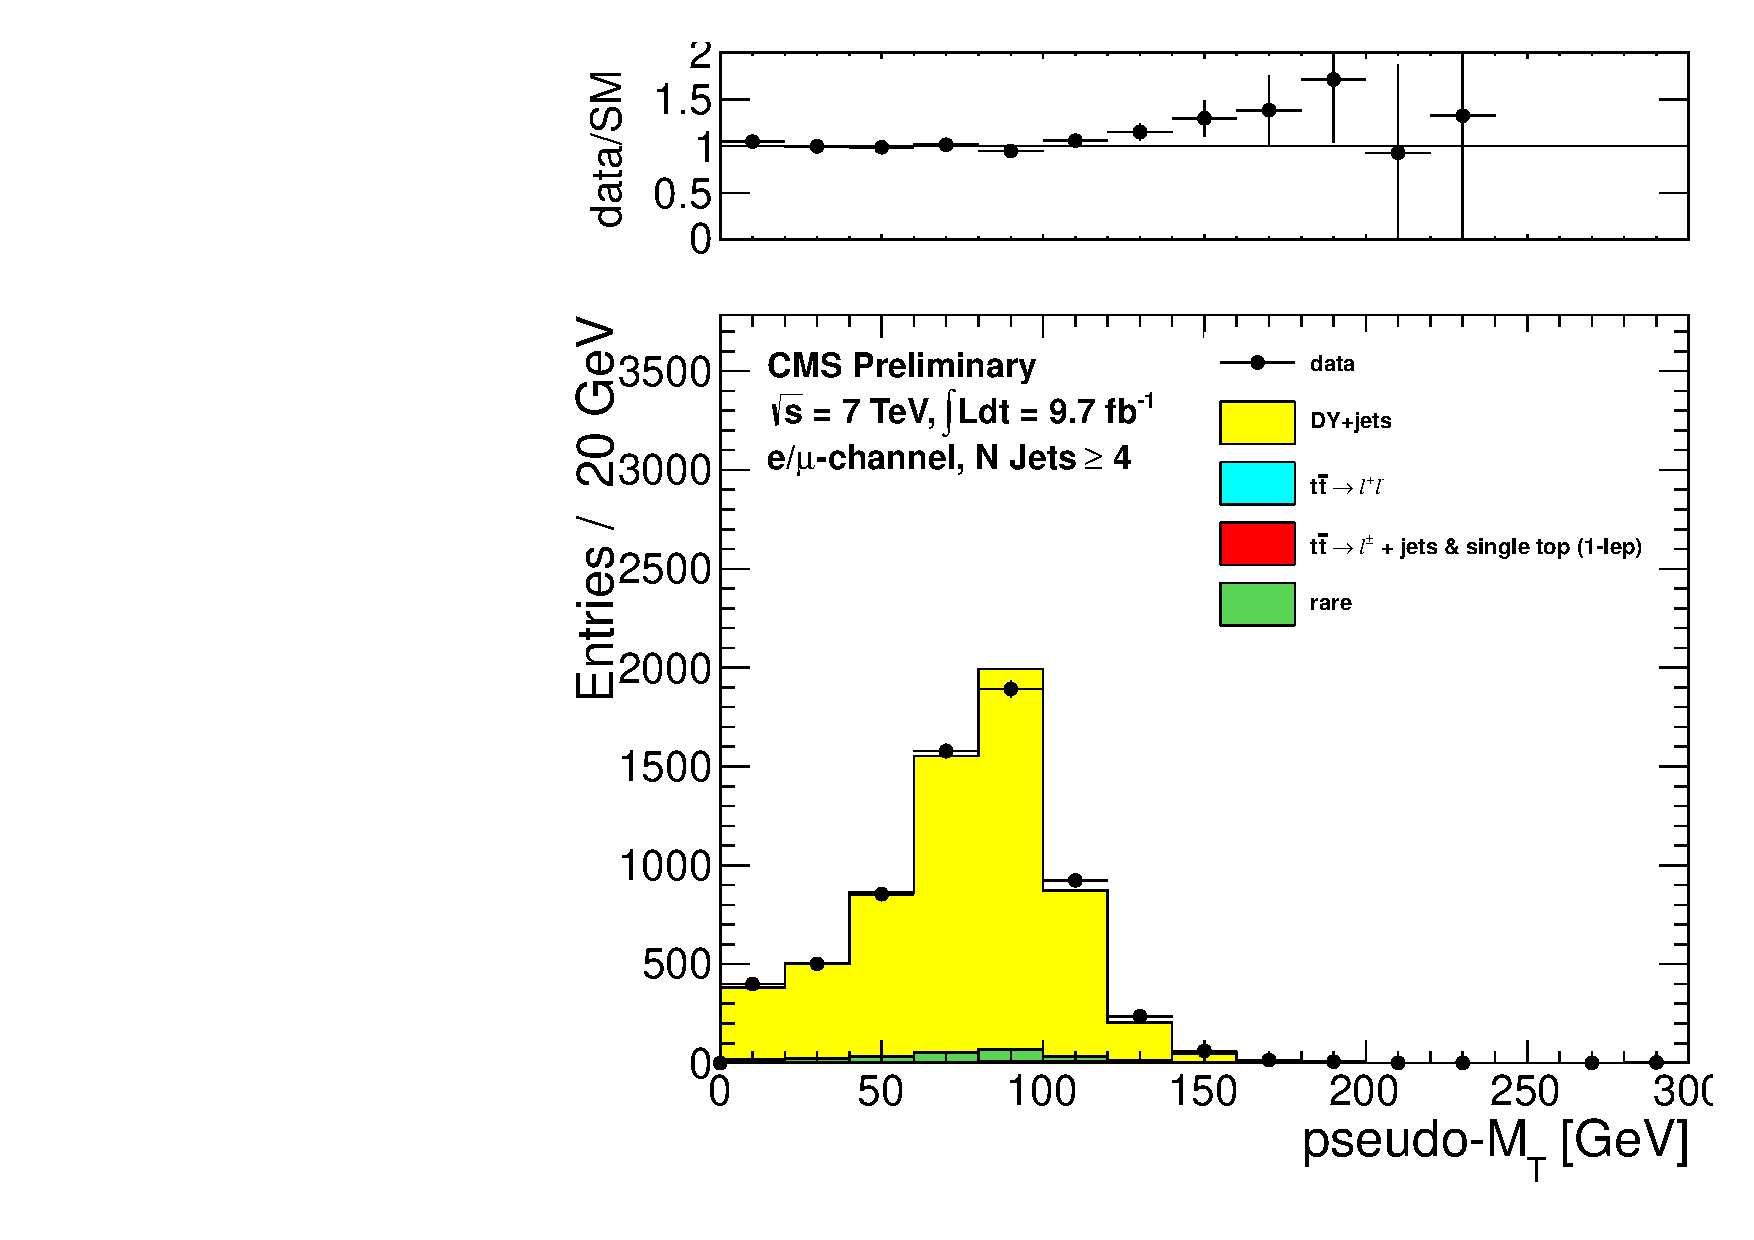
\includegraphics[width=0.5\linewidth]{plots/pas_lin/mt_lepcor_scaled_nj4_emucomb_CR2.pdf}
     \caption{
       Comparison of the pseudo-\met\ distribution (left) and the pseudo-\mt\ distribution (right)
       in data vs. MC for CR2.
       \label{fig:cr2met} 
     }  
   \end{center}
 \end{figure}
  
 \clearpage



